\documentclass[a4paper,12pt]{report}
% Paquetes necesarios para el documento
\usepackage{tikz}           % Para hacer diagramas
\usetikzlibrary{shapes.geometric, arrows.meta, positioning}
\usepackage{calc}           % Para realizar cálculos
\usepackage{float}          % Posición exacta de tablas e imágenes
\usepackage{hyperref}       % Enlaces dentro del PDF
\usepackage{pdfpages}       % Insertar PDFs
\usepackage{graphicx}       % Insertar gráficos e imágenes
\usepackage{tabularray}     % Tablas avanzadas
\usepackage{lscape}         % Páginas en orientación apaisada
\usepackage[spanish]{babel} % Configuración de idioma español
\usepackage{fancyhdr}       % Encabezados y pies de página
\usepackage{tocloft}        % Personalizar tabla de contenidos
\usepackage{setspace}       % Configurar espaciado
\usepackage{eso-pic}        % Insertar elementos de fondo
\usepackage{ragged2e}       % Control de alineación de texto
\usepackage{titlesec}       % Configuración de títulos de sección
\usepackage[table,xcdraw]{xcolor} % Colores avanzados
\usepackage{listings}       % Código fuente
\usepackage{rotating}       % Rotación de objetos
\usepackage[export]{adjustbox} % Ajuste de tamaño de imágenes
\usepackage{pdflscape}      % Orientación apaisada para algunas páginas
\usepackage{subcaption}     % Subfiguras
\usepackage{array}          % Tablas avanzadas
\usepackage{appendix}       % Apéndices
\usepackage{tabularx}       % Tablas con ancho fijo
\usepackage{enumitem}       % Listas personalizadas

% Definición de colores personalizados
\definecolor{celeste_rev}{HTML}{045bce}
\definecolor{verde_rev}{HTML}{52df28}
\definecolor{codeyellow}{rgb}{1,1,0}
\definecolor{codegreen}{rgb}{0,1,0}
\definecolor{codeblue}{rgb}{0.6,0.8,1}
\definecolor{backcolour}{rgb}{0.1,0.1,0.3}

% Configuración de hipervínculos
\hypersetup{
    colorlinks=true,
    linkcolor=celeste_rev,
    filecolor=red,
    urlcolor=verde_rev,
    pdftitle={Carpeta Técnica Rev-Control},
    pdfpagemode=FullScreen
}

% Definición del estilo para código fuente
\lstdefinestyle{mystyle}{
    backgroundcolor=\color{backcolour},
    commentstyle=\color{codegreen},
    keywordstyle=\color{codeyellow},
    numberstyle=\tiny\color{backcolour},
    stringstyle=\color{codeblue},
    basicstyle=\ttfamily\footnotesize\color{white},
    breaklines=true,
    captionpos=b,
    keepspaces=true,
    numbers=left,
    numbersep=5pt,
    showspaces=false,
    showstringspaces=false,
    showtabs=false,
    tabsize=2
}

\lstset{style=mystyle}

% Configuración de márgenes y encabezados
\usepackage[a4paper, margin=2.5cm]{geometry}
\pagestyle{fancy}
\fancyhf{}
\fancyhead[L]{Rev-Control}
\fancyhead[R]{\leftmark}
\fancyfoot[C]{\thepage}

% Formato de la tabla de contenidos
\renewcommand{\cftsecleader}{\cftdotfill{\cftdotsep}}

\begin{document}

% Imagen de fondo
\AddToShipoutPictureBG*{%
    \AtPageLowerLeft{%
        
\includegraphics[width=\paperwidth,height=\paperheight]{Imagenes/fondo3214 (2).png}
    }
}

% Carátula del documento
\begin{titlepage}
    \centering
    
\includegraphics[width=1.1\textwidth, height=2.3cm]{Imagenes/logos2.png}
    \vspace{1cm}
    
\includegraphics[width=0.7\textwidth]{Imagenes/LOGO REV CONTROL OFICIAL2.png}\\
    \vspace{1cm}
    {\Huge \textbf{\textcolor{celeste_rev}{Carpeta Técnica}}\\}
    \vspace{1cm}
    {\Large \textcolor{verde_rev}{Curso: 7° 1° Aviónica}}\\
    \vspace{0.5cm}
    {\Large \textcolor{celeste_rev}{Comisión: C}}\\
    \vspace{1cm}
    \textbf{\textcolor{celeste_rev}{Página web:}} \href{https://www.google.com/}{Link de acceso}\\
    \textbf{\textcolor{celeste_rev}{Trello:}} \href{https://trello.com/b/yDSPDlAp/kanban}{Link de acceso}\\
    \textbf{\textcolor{celeste_rev}{Github:}} \href{https://github.com/impatrq/revcontrol}{Link de acceso}\\
    \textbf{\textcolor{celeste_rev}{Redes Sociales:}} \href{https://www.instagram.com/rev.control/}{Link de acceso}\\
    \vfill
    \textbf{\textcolor{celeste_rev}{IMPA TRQ E.E.S.T N°7 2024}}\\
\end{titlepage}

% Tabla de contenidos
\tableofcontents
\newpage

% Inclusión de secciones
\chapter{Preámbulo}
    \section{Integrantes}
    
        \begin{itemize}
            \item Gonzalo Acosta
            \item Lautaro Alfaro
            \item Leonardo He
            \item Tadeo Ibaceta
            \item Marcos Martinez
            \item Juan Quintero
            \item Santiago Flores
        \end{itemize}
                    
    
    \section{Foto de cada integrante}
    Información\par
    
    \section{Foto grupal}
    Información\\
    
    \section{Horas dedicadas por cada integrante (registro personal)}
    Información\\
\chapter{Introducción}

\section{Objetivo}  
El objetivo de \textbf{REV-CONTROL} es ofrecer una solución innovadora y accesible para técnicos y mecánicos, permitiendo medir de manera eficiente y precisa los parámetros críticos de un motor. Este banco de prueba portátil, REV-CONTROL, facilita el diagnóstico y mantenimiento, utilizando tecnología de punta de amplificación y filtración de señales para proporcionar datos en tiempo real sobre las condiciones del motor.

\section{Descripción de la solución buscada}  
REV-CONTROL es un banco de prueba portátil diseñado para obtener datos precisos sobre los parámetros esenciales de cualquier motor. Con su diseño compacto y fácil de usar, REV-CONTROL está optimizado para realizar mediciones de revoluciones por minuto (RPM), presión y temperatura del aceite, temperatura de la cabeza de cilindro, temperatura de agua y concentración de oxígeno en los gases. Su sistema permite a los técnicos tomar decisiones rápidas y acertadas para garantizar el correcto funcionamiento de los motores.

\section{Segmento destino y alcance}  
El público objetivo de \textbf{REV-CONTROL} son los técnicos y mecánicos que trabajan en mantenimiento y diagnóstico de motores, desde vehículos de carretera hasta equipos industriales. Con un alcance global, este sistema busca transformar el modo en que se gestionan las pruebas de motor, especialmente en situaciones donde la portabilidad, la rapidez y la precisión son esenciales.

\section{Captura representativa del proyecto}

\begin{figure}[H]
    \centering
    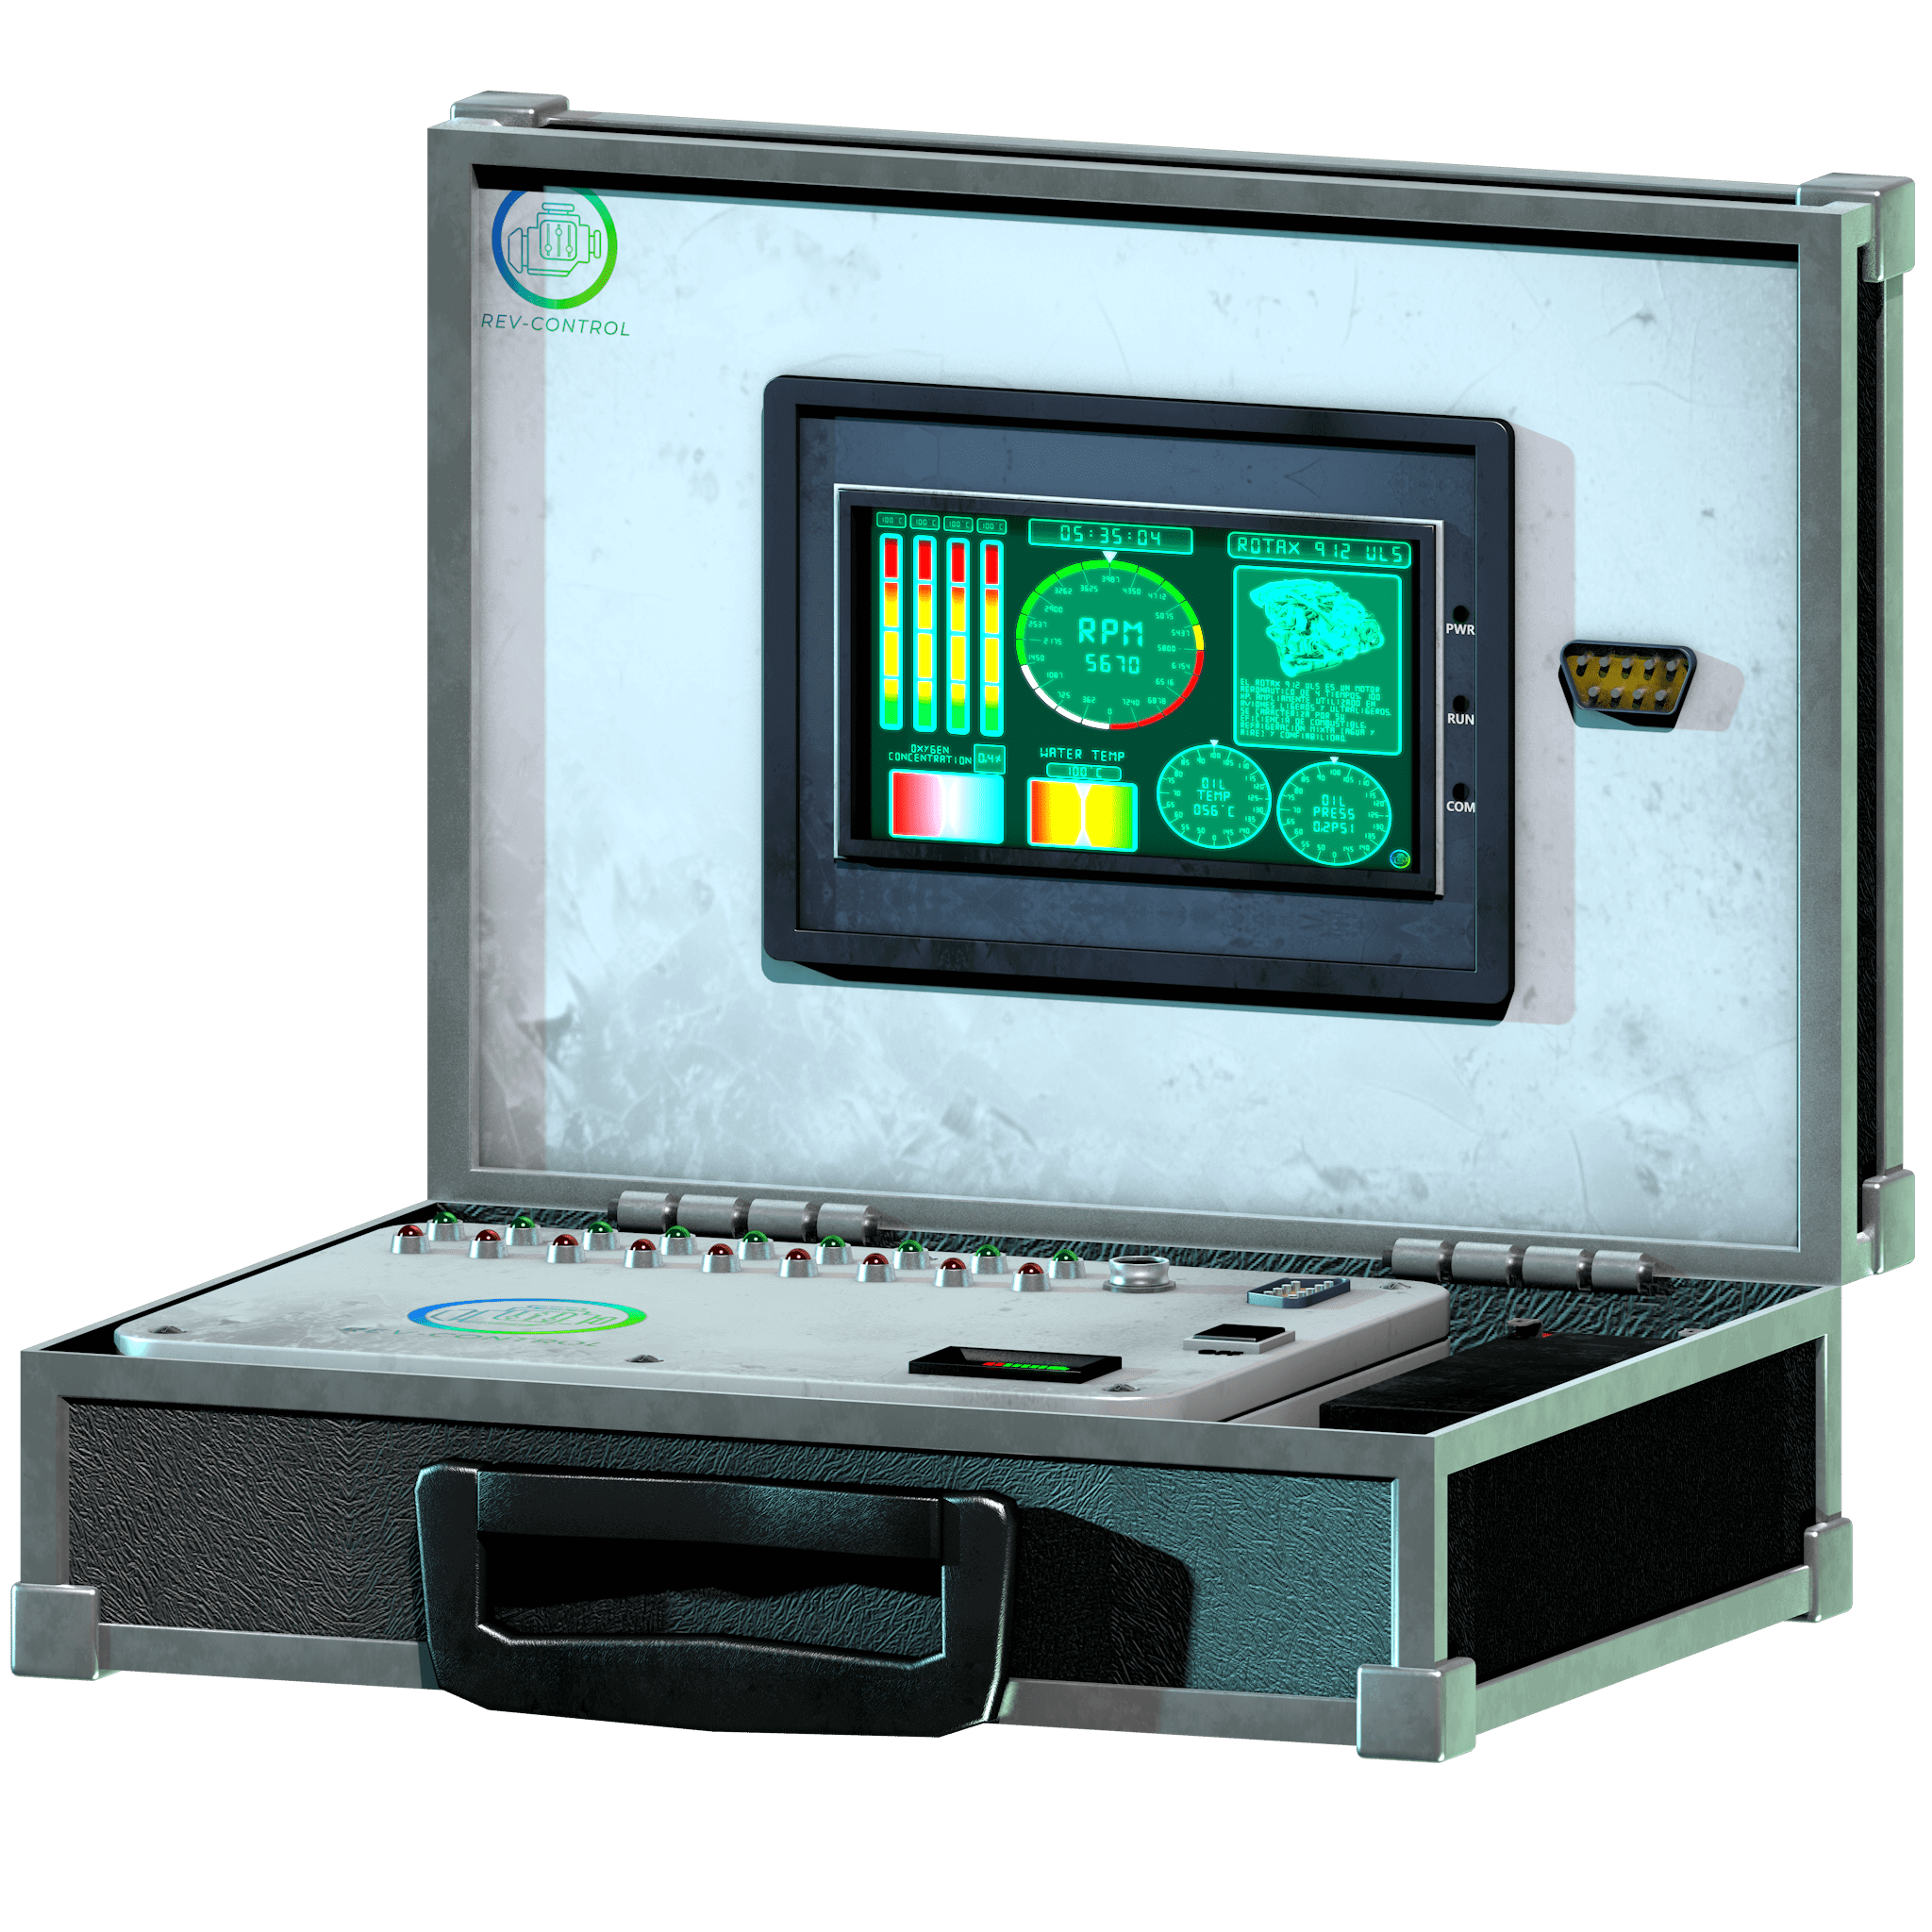
\includegraphics[width=0.6\textwidth]{Imagenes/Monitor y maletin-min.png}
    \caption{Imagen representativa del proyecto REV-CONTROL en funcionamiento.}
    \label{fig:representativa}
\end{figure}

\section{Diagrama en bloques del proyecto}

\begin{figure}[H]
    \centering
    \begin{tikzpicture}[
      block/.style={rectangle, draw, text centered, minimum height=1cm, minimum width=3cm, rounded corners},
      arrow/.style={-{Latex[length=3mm, width=2mm]}, thick},
      node distance=1.5cm
    ]
      
      % Definición de nodos
      \node[block, fill=cyan!30] (motor) {Motor en funcionamiento};
      \node[block, fill=green!30, below=of motor] (sensores) {Sensores de parámetros críticos};
      \node[block, fill=blue!30, below=of sensores] (condicionamiento) {Condicionamiento de señales};
      \node[block, fill=cyan!30, below=of condicionamiento] (lpc845) {Microcontrolador LPC845};
      \node[block, fill=green!30, below=of lpc845] (alarma) {Sistema de alarma};
      \node[block, fill=green!30, right=of lpc845] (monitor) {Monitor Kinseal};

      % Conexiones con flechas
      \draw[arrow] (motor) -- (sensores);
      \draw[arrow] (sensores) -- (condicionamiento);
      \draw[arrow] (condicionamiento) -- (lpc845);
      \draw[arrow] (lpc845) -- (alarma);
      \draw[arrow] (lpc845) -- (monitor);

    \end{tikzpicture}
    \caption{Diagrama en bloques del sistema REV-CONTROL.}
    \label{fig:diagrama_bloques}
\end{figure}

\section{Motor utilizado en el proyecto (ROTAX 912 ULS)}

El \textbf{\href{https://www.flyrotax.com/products/912-uls-s}{Rotax 912 ULS}} es un motor de cuatro tiempos ampliamente utilizado en aeronaves ligeras, vehículos todoterreno y aplicaciones industriales.  
\begin{itemize}
    \item Configuración: Motor bóxer de 4 cilindros, refrigerado por líquido y aire.  
    \item Cilindrada: 1,352 cm³.  
    \item Potencia: 100 HP (73.5 kW) a 5,800 RPM.  
    \item Alimentación: Sistema de carburadores duales.  
    \item Características destacadas: Alta fiabilidad, bajo peso, eficiencia de combustible y capacidad para operar con gasolina sin plomo.  
    \item Aplicación en el proyecto: Recolección y análisis de datos críticos como temperatura, presión de aceite, proporción aire-combustible y velocidad de rotación.  
\end{itemize}

\begin{figure}[H]
    \centering
    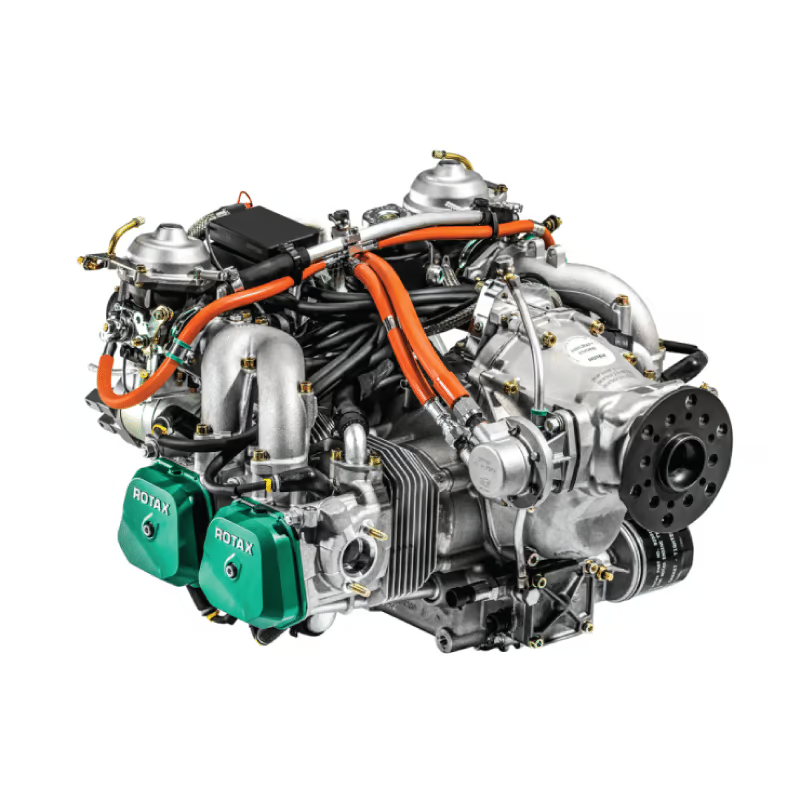
\includegraphics[width=0.8\textwidth]{Imagenes/ROTAX.png}
    \caption{Motor Rotax 912 ULS}
    \label{fig:motor_rotax_912}
\end{figure}


\section{Resultado conseguido}  
El resultado de \textbf{REV-CONTROL} es una herramienta integral para diagnóstico de motores, que ofrece mediciones precisas y en tiempo real de parámetros críticos. Su sistema permite a los técnicos obtener datos detallados de manera clara y sencilla, mejorando la eficacia en las reparaciones y mantenimiento de motores, además de ofrecer un sistema de alarmas para alertar de situaciones críticas en los parámetros monitoreados.

\chapter{Software}

\section{Códigos significativos}
A continuación se adjunta el código de lectura de pines en \hyperref[adc_code]{ADC} y \hyperref[spi_code]{SPI}:

% Fragmento de código ADC
\lstinputlisting[
    language=C,
    caption=Lectura de ADC, 
    label=adc.code
]{rev-control_adc.c}

% Fragmento de código SPI
\lstinputlisting[
    language=C,
    caption=Lectura de SPI, 
    label=spi.code
]{rev-control_spi.c}
    
    \section{Capturas de interfaces visuales}
        Información
    
    \section{Estructuras de datos}

Esta sección describe las principales estructuras de datos utilizadas para gestionar las lecturas de los sensores y la comunicación SPI en el sistema. Se incluye una descripción de las variables globales, las funciones clave, y las estructuras de configuración para el ADC y el SPI.

\subsection{Variables globales}

Las variables globales se emplean para almacenar la configuración y los resultados de las conversiones ADC y SPI. A continuación, se describen las más importantes:

\begin{itemize}
    \item \textbf{adc\_channel[3]}: Un \textit{array} de 8 bits que define los canales ADC en uso. Cada elemento representa un canal específico:
        \begin{itemize}
            \item \texttt{ADC0\_CH1}: Canal para la concentración de oxígeno.
            \item \texttt{ADC0\_CH2}: Canal para las RPM.
            \item \texttt{ADC0\_CH3}: Canal para la presión de aceite.
        \end{itemize}
        
    \item \textbf{channel\_result[3]}: Un \textit{array} de enteros de 16 bits que almacena los resultados de la conversión ADC para cada canal.

    \item \textbf{lambda}, \textbf{oil\_pressure}, \textbf{RPM}: Variables de 16 bits donde se guardan los valores procesados de cada lectura del canal, correspondientes a la concentración de oxígeno, la presión de aceite y las RPM, respectivamente.

    \item \textbf{CS[7]}: Un \textit{array} de enteros de 8 bits que representa los pines de Chip Select (CS) utilizados para manejar distintos dispositivos SPI conectados al sistema.
\end{itemize}

\subsection{Funciones y prototipos principales}

Estas funciones organizan el flujo del programa, facilitando la adquisición y transmisión de datos desde los sensores al sistema:

\begin{itemize}
    \item \textbf{void ADC\_Configuration(void)}: Configura el ADC, activando los canales necesarios y definiendo los parámetros de conversión.

    \item \textbf{void spi\_cs\_low(void)} y \textbf{void spi\_cs\_high(void)}: Controlan el estado de los pines de Chip Select (CS) para habilitar o deshabilitar el dispositivo SPI según sea necesario.

    \item \textbf{float max6675\_get\_temp(void)}: Realiza una lectura de temperatura desde un sensor MAX6675 a través de SPI, devuelve el valor en grados Celsius.
\end{itemize}

\subsection{Estructura de configuración para el SPI}

La estructura \texttt{spi\_transfer\_t} se utiliza para definir los parámetros de la transferencia SPI. Esto organiza la lectura del sensor de temperatura y otros dispositivos conectados:

\begin{itemize}
    \item \texttt{txData}: Puntero a los datos que se van a transmitir (NULL si no se envían datos).
    \item \texttt{rxData}: Puntero a los datos recibidos en la transferencia.
    \item \texttt{dataSize}: Tamaño de la transferencia en bytes (en este caso, 2 bytes).
    \item \texttt{configFlags}: Indicadores de configuración que controlan la finalización de la transferencia y el formato de los datos.
\end{itemize}

\subsection{Estructura de configuración para el ADC}

La estructura \texttt{adc\_conv\_seq\_config\_t} define el modo de conversión y los canales activos para el ADC. Los campos principales son:

\begin{itemize}
    \item \texttt{channelMask}: Máscara de bits que activa los canales especificados en el ADC.
    \item \texttt{triggerMask}: Define el disparo de conversión, ya sea en modo automático o por software.
    \item \texttt{interruptMode}: Configura las interrupciones que se activan cuando la conversión en un canal finaliza.
\end{itemize}

Estas estructuras de datos, variables y funciones permiten un manejo organizado y eficiente de las lecturas y configuraciones de los sensores en el sistema embebido.

 

    
\chapter{Sistema embebido}

\section{Microcontroladores y/o microprocesadores utilizados}
En este proyecto, el microcontrolador LPC845 actúa como el núcleo de procesamiento central, manejando y coordinando la información que proviene de diversos sensores y periféricos. Este microcontrolador, basado en la arquitectura ARM Cortex-M0+, es seleccionado por su eficiencia energética y capacidad de realizar múltiples tareas de forma simultánea. A través de sus múltiples puertos de comunicación, el LPC845 se conecta con los componentes periféricos y transmite datos de estado directamente al Kinseal AMZ070W01RAGD, una pantalla que permite la visualización en tiempo real para el usuario. La interacción entre el LPC845 y el Kinseal es fundamental para la interfaz de usuario, ya que permite al operador monitorear el funcionamiento del sistema.

\section{Placas de desarrollo}
La placa de desarrollo empleada es la LPC845-BRK, una plataforma compacta que permite la rápida evaluación y desarrollo de aplicaciones basadas en el microcontrolador LPC845. La placa incluye una interfaz de depuración integrada, soporte para periféricos digitales y analógicos, y un puerto micro-USB para comunicación y programación. Este diseño compacto permite el acceso directo a los pines del microcontrolador, ideal para experimentación con módulos SPI y ADC. Esta configuración permite la conexión física con el Kinseal AMZ070W01RAGD, lo que facilita la implementación de la interfaz gráfica de usuario. Además, la placa proporciona estabilidad y protección a los circuitos, asegurando una transmisión de datos confiable entre el LPC845 y los periféricos.

\section{Software utilizados para el desarrollo}
El desarrollo de este sistema embebido se llevó a cabo con MCUXpresso IDE, un entorno de desarrollo integrado (IDE) específico para microcontroladores NXP. MCUXpresso proporciona herramientas avanzadas para depuración, control de periféricos y optimización de código en C/C++. Para la compilación y enlace del código, se empleó el compilador GNU ARM Toolchain compatible con la arquitectura Cortex-M0+. Además, se utilizó la biblioteca SDK de NXP que facilita la configuración de periféricos, manejo de GPIO, y control del módulo ADC y SPI. Además, para la configuración de la interfaz gráfica del Kinseal AMZ070W01RAGD, se emplearon los programas HMILite 2.22 y Kinseal Studio, diseñados para crear y gestionar interfaces HMI. HMILite 2.22 facilita la visualización en tiempo real de datos procesados, mientras que Kinseal Studio permite diseñar la interfaz gráfica que conecta al usuario con el sistema embebido.

\section{Diagrama en bloque de la solución}

    \begin{figure}[h]
        \centering
        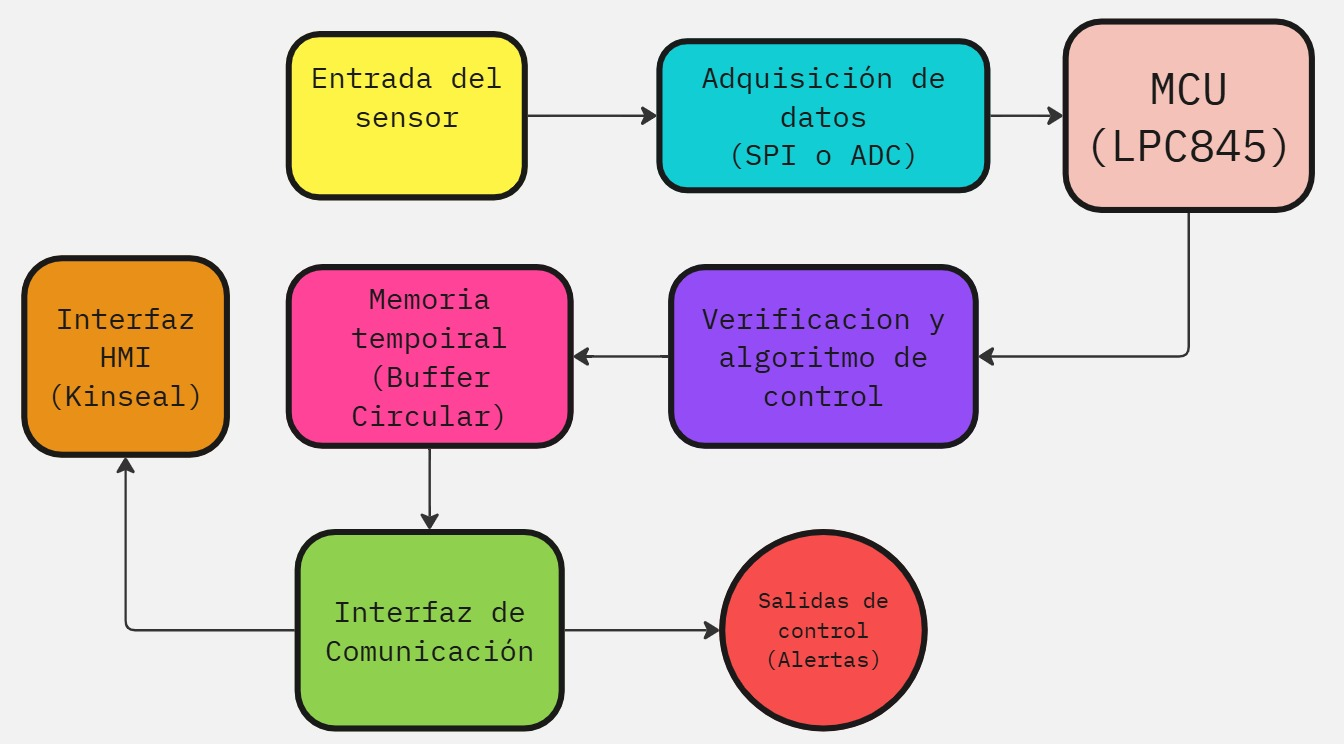
\includegraphics[width=0.8\textwidth]{Imagenes/Diagrama en bloques de sistema embibido.jpg}
        \caption{Diagrama en bloque de la solución}
        \label{fig:diagrama_bloque}
    \end{figure}

\section{Lenguajes de programación usados}
El sistema fue programado en C, un lenguaje de programación estructurado que es ampliamente utilizado en el desarrollo de sistemas embebidos por su eficiencia y control sobre el hardware. Las bibliotecas específicas de NXP permiten gestionar de manera eficiente los periféricos integrados, y el código está optimizado para la arquitectura ARM Cortex-M0+ del LPC845, garantizando un rendimiento adecuado en tiempo real. Para el desarrollo de la interfaz gráfica en el Kinseal AMZ070W01RAGD, Kinseal Studio permite el uso de un lenguaje de scripting específico para HMI, que facilita la creación de elementos gráficos y lógica de control en pantalla. Este lenguaje permite configurar la visualización de datos y ajustar la interactividad del sistema de manera personalizada, adaptándose a los requisitos del proyecto y logrando una interfaz amigable para el usuario.

\section{Especificación de periféricos utilizados}

\begin{itemize}
    \item \textbf{SPI (Serial Peripheral Interface):} Protocolo de comunicación utilizado para interactuar con el sensor de temperatura MAX6675. El SPI permite leer valores de temperatura en tiempo real y se configura con un reloj SCK de 1 MHz y distintos pines de selección de chip.
    
    \item \textbf{ADC (Analog-to-Digital Converter):} El sistema utiliza un ADC de 12 bits para leer valores analógicos de sensores de concentración de oxígeno, RPM y presión de aceite. Con un voltaje de referencia de 3.3V, el ADC convierte las señales analógicas en valores digitales, proporcionando precisión en la captura de datos del entorno.
    
    \item \textbf{GPIO (General-Purpose Input/Output):} Los pines GPIO permiten configurar salidas para el control de periféricos y selección de chips, activando y desactivando los pines CS de cada módulo.
\end{itemize}

\section{Estructuras de datos}

El sistema embebido utiliza una estructura de datos organizada y eficiente para almacenar, procesar y manejar la información recibida de los distintos sensores. Este diseño facilita el procesamiento en tiempo real, optimizando la memoria y permitiendo que el sistema mantenga datos consistentes y de fácil acceso. A continuación, se detallan las estructuras de datos utilizadas:

\subsection{Struct para sensores individuales}

Se define una estructura \texttt{SensorData} para cada sensor, que contiene campos específicos para cada medición. Esta estructura incluye los siguientes parámetros:

\begin{itemize}
    \item \texttt{float lectura}: valor de lectura convertido de datos analógicos a unidades físicas (°C para temperatura, rpm, bar para presión).
    \item \texttt{uint32\_t timestamp}: marca de tiempo para la toma de cada lectura, asegurando la sincronización en el procesamiento.
    \item \texttt{bool estado}: indicador de estado para verificar si la lectura es válida o si ha habido un error en el sensor.
\end{itemize}

\subsection{Especificación de periféricos utilizados}

En este sistema, los periféricos son esenciales para la adquisición y comunicación de datos críticos para el control del sistema embebido y su interfaz gráfica con el usuario. A continuación, se detallan los periféricos clave utilizados:

\begin{itemize}
    \item \textbf{MAX6675}: Este sensor se utiliza para medir la temperatura en las termocuplas de cabeza de cilindro. Proporciona datos de temperatura precisos y confiables mediante la interfaz SPI, lo que permite un monitoreo efectivo de las condiciones térmicas del motor.
    
    \item \textbf{MAX31865}: Se utiliza para los termistores de aceite y de agua. Este conversor RTD convierte la resistencia del termistor a una lectura digital precisa, proporcionando datos de alta precisión para el monitoreo de la temperatura del aceite y del agua en el sistema. La comunicación con el LPC845 se realiza a través de la interfaz SPI.

    \item \textbf{Sensor de presión de aceite}: Este sensor mide la presión en el sistema de aceite, proporcionando información esencial para el monitoreo del motor. La comunicación se realiza a través de la entrada ADC del LPC845.

    \item \textbf{Sensor de concentración de oxígeno}: Captura los niveles de oxígeno y se comunica con el microcontrolador para ofrecer datos críticos sobre la combustión y otros parámetros ambientales. Este sensor también se conecta mediante la interfaz ADC.

    \item \textbf{Sensor de RPM}: Este sensor permite la lectura de la velocidad del motor en revoluciones por minuto (RPM). Utiliza la entrada ADC del LPC845 para medir la señal analógica proporcional a la velocidad del motor, proporcionando lecturas en tiempo real. Esta configuración garantiza una alta precisión en el monitoreo de RPM y permite ajustar la respuesta del sistema en función de la velocidad del motor.

    \item \textbf{Comunicación con Kinseal AMZ070W01RAGD}: La pantalla táctil Kinseal está conectada al sistema mediante comunicación serial UART. A través de este canal, el LPC845 envía información de cada sensor y recibe comandos, actualizando en tiempo real la interfaz gráfica desarrollada en Kinseal Studio con el software HMILite 2.22.
\end{itemize}

Esta combinación de periféricos asegura que el sistema embebido capture, procese y comunique los datos relevantes, permitiendo una visualización y control eficientes en el dispositivo HMI.

\chapter{Electrónica}

\section{Diagrama en bloque de las partes}
Información

\section{Software usado para el desarrollo de esquemáticos y PCB}
Información

\section{Esquemático de cada bloque}
Información

\section{PCB de cada bloque}
Información

\section{Modelo 3D de cada PCB}
Información

\section{Especificaciones sobre fuentes de alimentación y potencias}
Información

\section{Especificaciones técnicas de los componentes}
Información
\chapter{Estructura}

\section{Diagrama general de la estructura}

      \begin{figure}[H]
    \centering
    \begin{tikzpicture}[line width=2pt, rounded corners, every node/.style={font=\sffamily, draw, minimum width=1.5cm, minimum height=1cm, align=center}]
        
        % Colores personalizados
        \definecolor{colorEntrada}{RGB}{173, 216, 230} % Azul claro para entradas
        \definecolor{colorIntermedio}{RGB}{255, 228, 181} % Amarillo claro para nodos A y B
        \definecolor{colorSalida}{RGB}{144, 238, 144} % Verde claro para el nodo C
        
        % Colores para las flechas
        \definecolor{colorFlechaEntrada}{RGB}{100, 149, 237} % Azul para flechas de entrada
        \definecolor{colorFlechaIntermedio}{RGB}{255, 99, 71} % Rojo para flechas intermedias
        \definecolor{colorFlechaSalida}{RGB}{34, 139, 34} % Verde para flechas de salida
        \definecolor{colorFlechaMorada}{RGB}{128, 0, 128} % Morado para la flecha de entrada 1
        
        % Nodos (bloques) con las modificaciones
        \node[fill=colorEntrada] (entrada1) at (-4, 2) {Lado Inferior};
        \node[fill=colorEntrada] (entrada2) at (-4, -3) {Lado Superior};
        \node[fill=colorIntermedio] (A) at (0, 2) {Batería 12V 7AH}; % Batería más cerca
        \node[fill=colorIntermedio] (B) at (0, -2) {Módulo de Lectura}; % Módulo más cerca
        \node[fill=colorSalida] (C) at (6, 0) {Monitor};
        
        % Caja discontinua más grande en altura alrededor de A y B
        \draw[dashed, thick] (-2, 3) rectangle (2, -3); % Caja más grande
        
        % Conexiones con colores para las flechas, con mayor grosor
        \draw[color=colorFlechaMorada, line width=2pt, bend left=45] (entrada1) to (-2, 3); % Flecha morada curva
        \draw[color=colorFlechaEntrada, line width=2pt] (entrada2) -- ++(0, -1) -| (C); % Flecha de entrada 2 por abajo
        \draw[color=colorFlechaIntermedio, line width=2pt] (A) -- (C); % Flecha de A a C recta
        \draw[ color=colorFlechaIntermedio, line width=2pt] (B) -- (C); % Flecha de B a C recta
        
    \end{tikzpicture}
    \begin{center}
    \caption{Diagrama en bloques de la estructura de Rev-Control.}
    \label{fig:diagrama_bloques_estruc}
    \vspace{0.5cm} % Espacio entre el caption y la nota
    \small{Nota: El módulo de lectura está conectado al monitor mediante el cable RS232.}
    \end{center}
    \end{figure}


\section{Software de diseño utilizado}
    \noindent  % Evita el sangrado de la sección
        \begin{center}
            
\includegraphics[width=0.2\textwidth]{Imagenes/cinema-4d-logo.png}
            \captionof{figure}{Cinema4D}
            \label{fig:logo_cinema}
        \end{center}
    
    \noindent Cinema 4D es un software de modelado, animación y renderizado 3D desarrollado por Maxon. Es ampliamente utilizado en la industria del diseño gráfico, efectos visuales y producción de películas. Con su interfaz intuitiva y potentes herramientas, Cinema 4D permite a los diseñadores crear modelos 3D detallados, animaciones complejas, simulaciones de físicas realistas y efectos visuales de alta calidad. La capacidad de integrar con otros programas de diseño y su versatilidad lo convierten en una opción popular entre los profesionales de la animación y el modelado 3D.

\section{Descripción de cada parte de la estructura}

\begin{itemize}

    \item \textbf{Maletín:} Es una opción de almacenamiento robusta y resistente, ideal para transportar equipos y herramientas en condiciones exigentes. Fabricado con materiales de alta calidad, ofrece protección contra impactos, agua y polvo. Su diseño incluye cierres seguros, asas ergonómicas y una estructura interna personalizable para organizar el contenido. Las paredes internas estan hechas de madera y los bordes de aluminio.
    
    \item \textbf{Monitor KINSEAL:} El Kinseal AMZ070W01RAGD es una pantalla táctil HMI industrial de 7 pulgadas, diseñada para aplicaciones que requieren un rendimiento robusto. Soporta interfaces de comunicación como RS232, RS485 y RS422, y opera con un rango de voltaje DC de 10-30V. Su pantalla tiene una resolución de 800x480 y una luminosidad de 450 cd/m², con una pantalla táctil resistiva de 4 hilos. Además, cuenta con 128MB de almacenamiento SPI NAND y puertos USB para transferencia de datos y descarga de programas. Su panel frontal tiene clasificación IP65.
    
    \item \textbf{Módulo de lectura:} Aqui estan los circuitos, conexiones y el cerebro del proyecto, El LPC845, donde esta todo lo necesario para usar Rev-Control. El modulo de lectura usa de base una caja modelo  Estanca 6 - Codigo: CE6 (Medidas: 300x210x80).
    
    \item \textbf{Batería de 12V:} La batería de plomo ácido gel es una batería sellada de 12 voltios y 7.0 Ah (amperios-hora), diseñada para ofrecer una alta fiabilidad y rendimiento en aplicaciones de respaldo de energía y sistemas de seguridad. Utiliza tecnología de gel, lo que la hace más resistente a las vibraciones y evita fugas de ácido, lo que la hace más segura y duradera. Es ideal para dispositivos como UPS, alarmas, sistemas solares y otros equipos que requieren energía confiable y constante.
    
\end{itemize}



\section{Imágenes exportadas de los diseños}
    
    \begin{itemize}
        \item \textbf{Diseño de maletín:} Recreación del maletín estilo ambil para ilustración.
        \begin{center}
            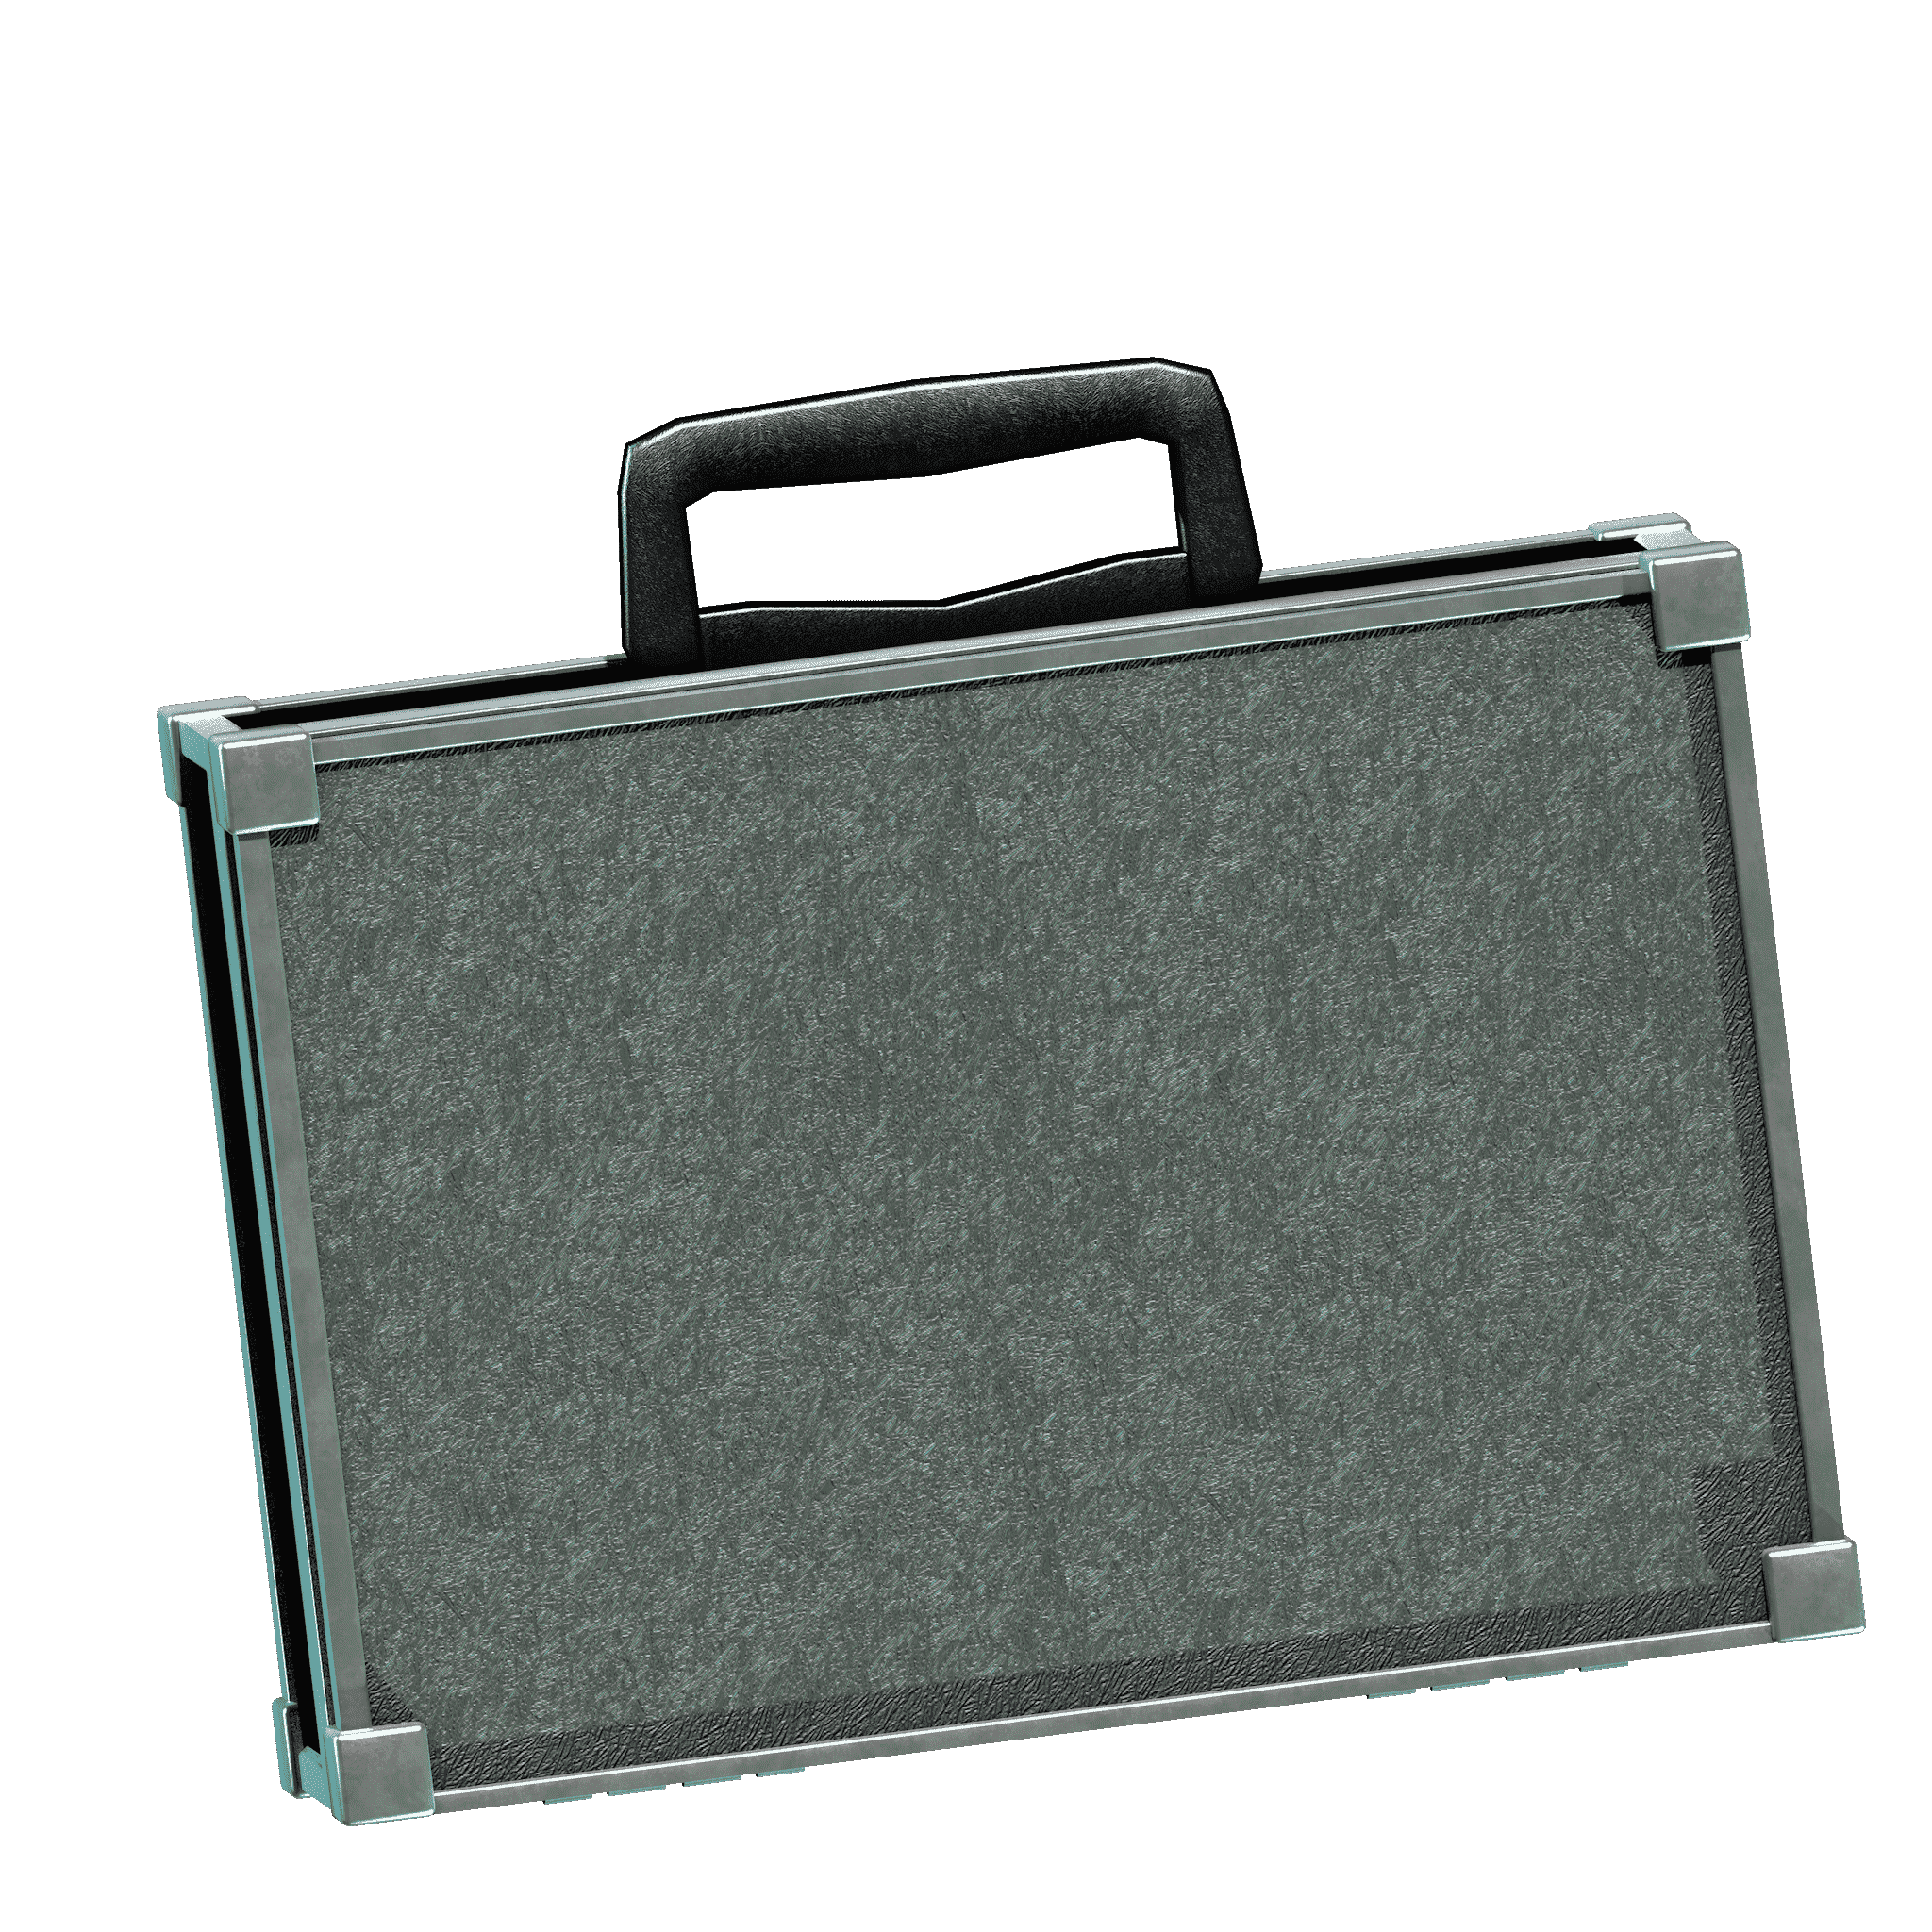
\includegraphics[width=0.8\textwidth]{Imagenes/Monitor y maletin42134.png}
            \captionof{figure}{Diseño de maletín}
            \label{fig:imagen1}
        \end{center}
        
        \item \textbf{Maletín abierto mostrando la interfaz digital:} Se usó un maletín estilo ambil para contener el módulo de lectura de datos y una batería de 12V 70Ah junto al monitor Kinseal en la tapa del maletín para visualizar su lectura.
        \begin{center}
            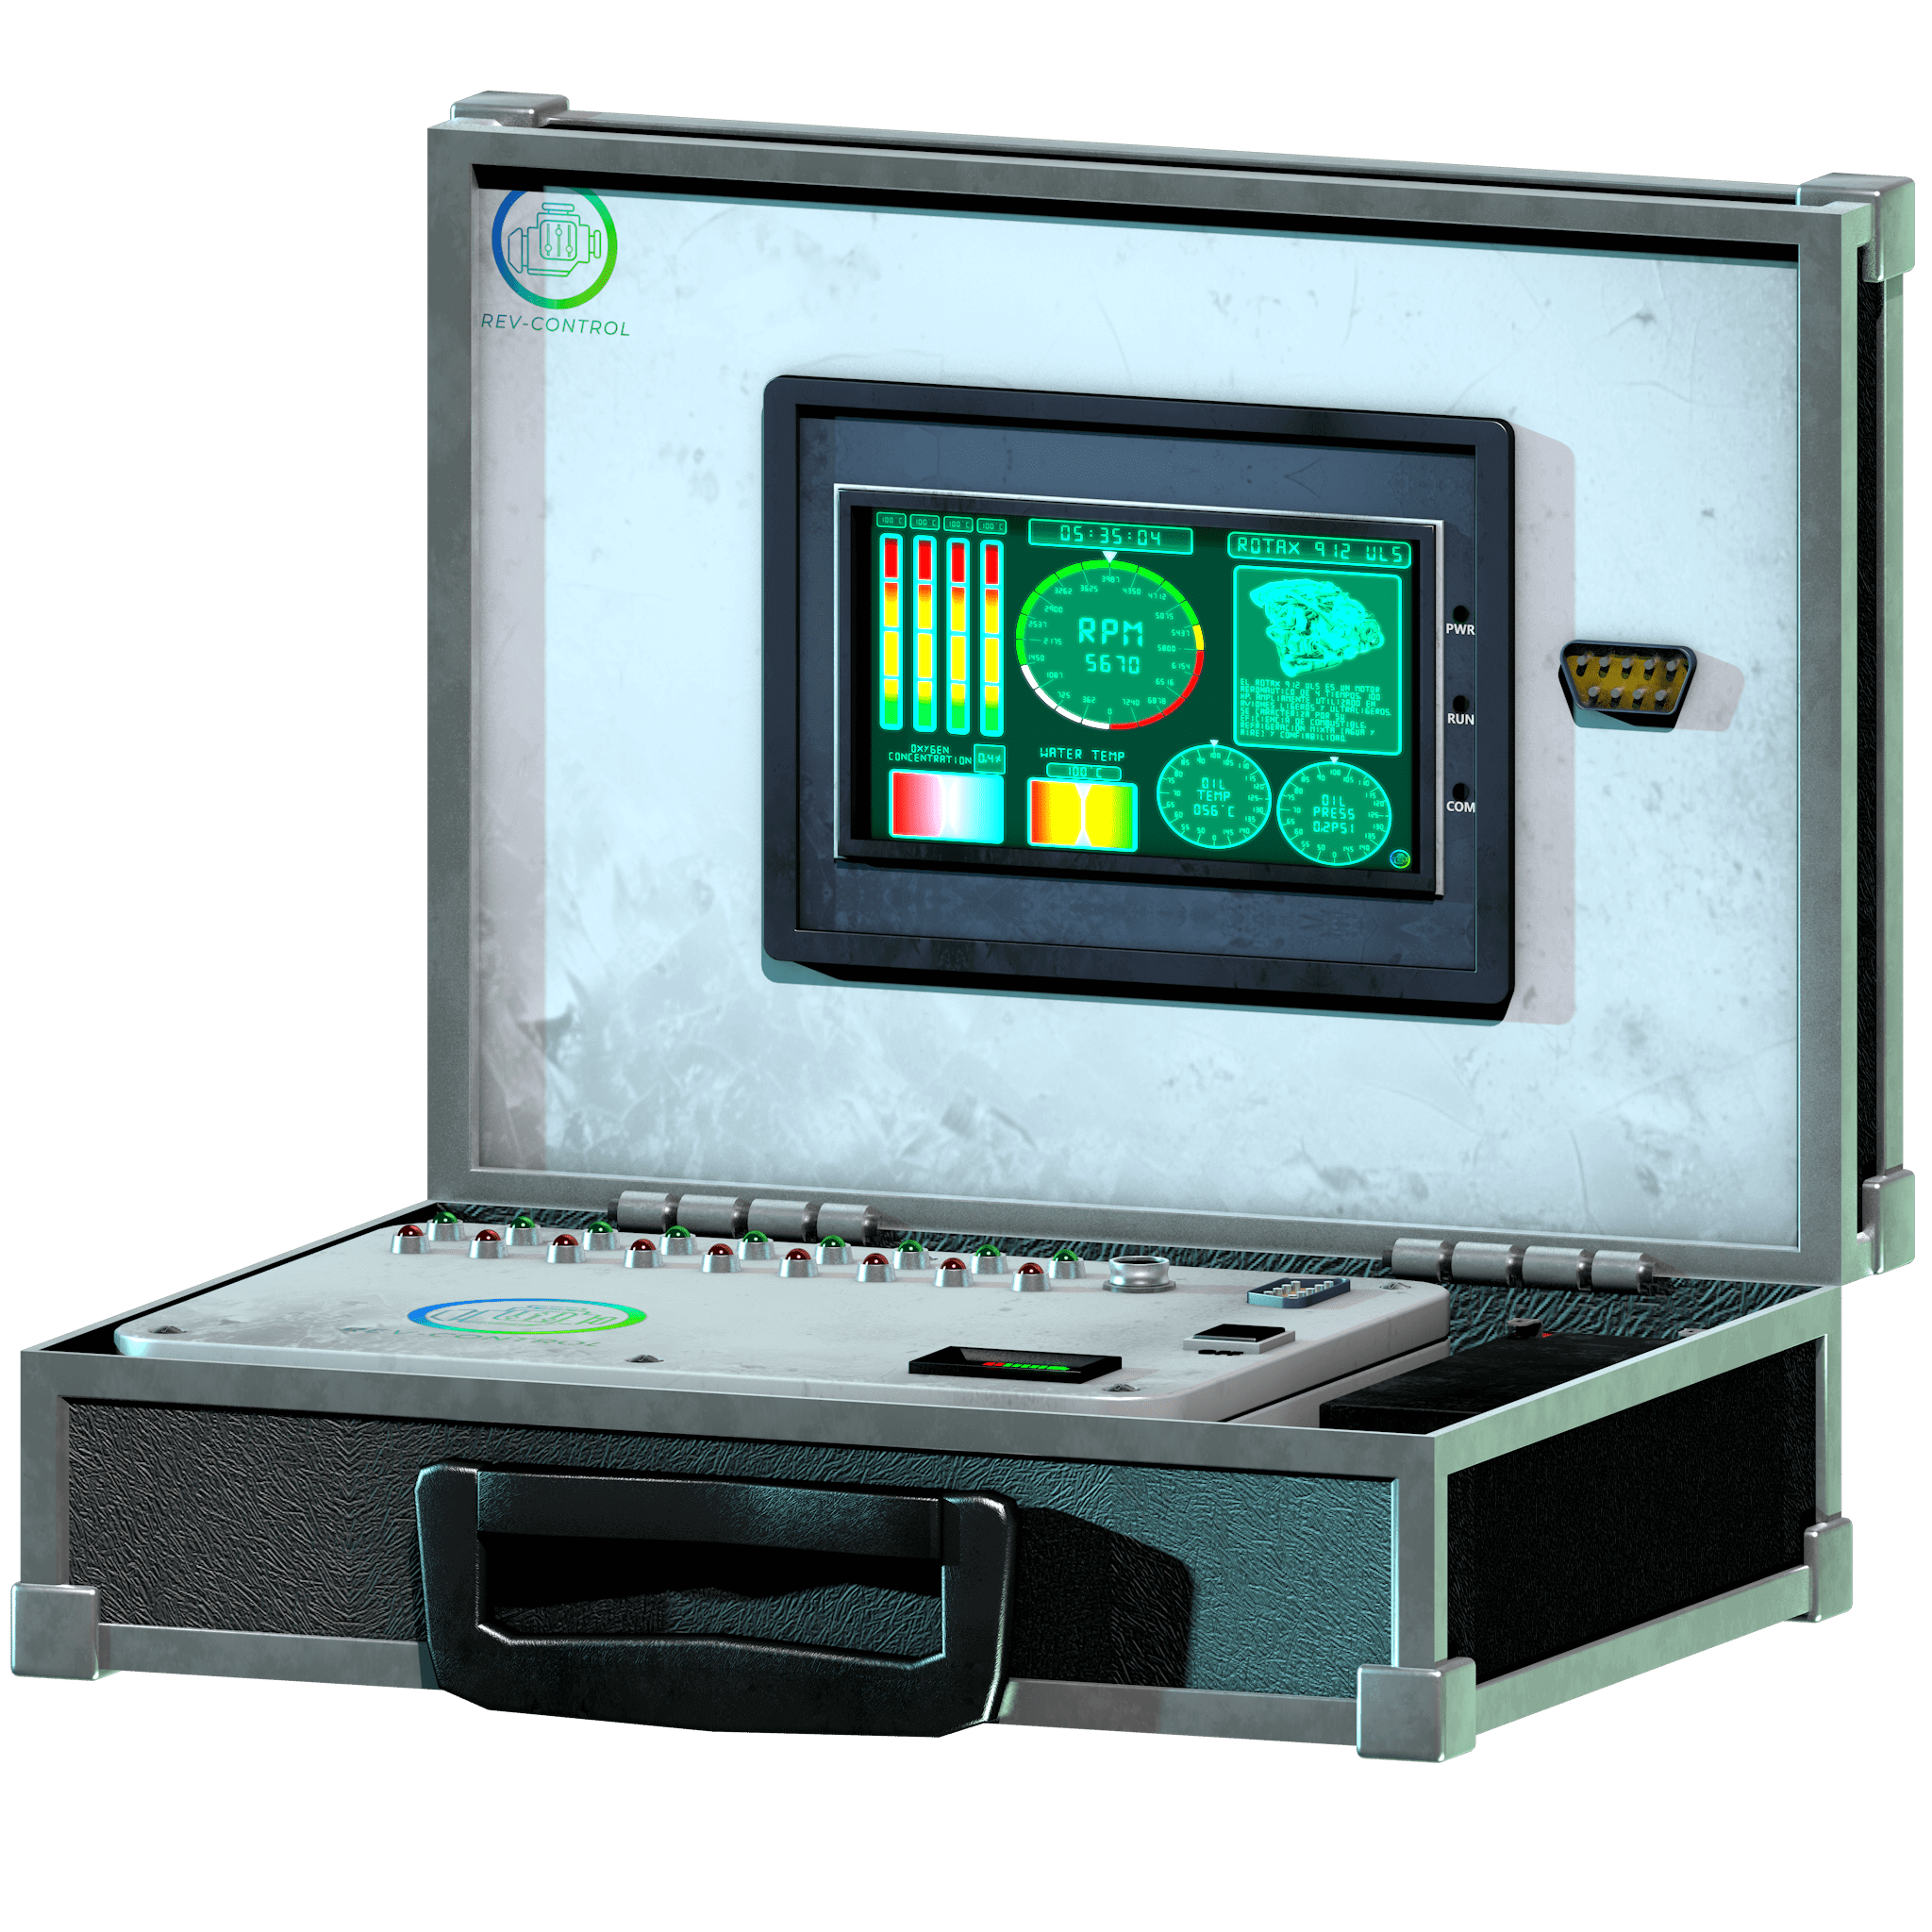
\includegraphics[width=0.8\textwidth]{Imagenes/Monitor y maletin-min.png}
            \captionof{figure}{Maletín abierto mostrando la interfaz digital}
            \label{fig:imagen2}
        \end{center}
        
        \item \textbf{Módulo de lectura de datos:} Este tiene las alarmas ojos de buey, un buzzer, un conector RS232, un switch de encendido, un voltímetro para mostrar la alimentación de la batería y atrás los conectores de cada sensor.
        \begin{center}
            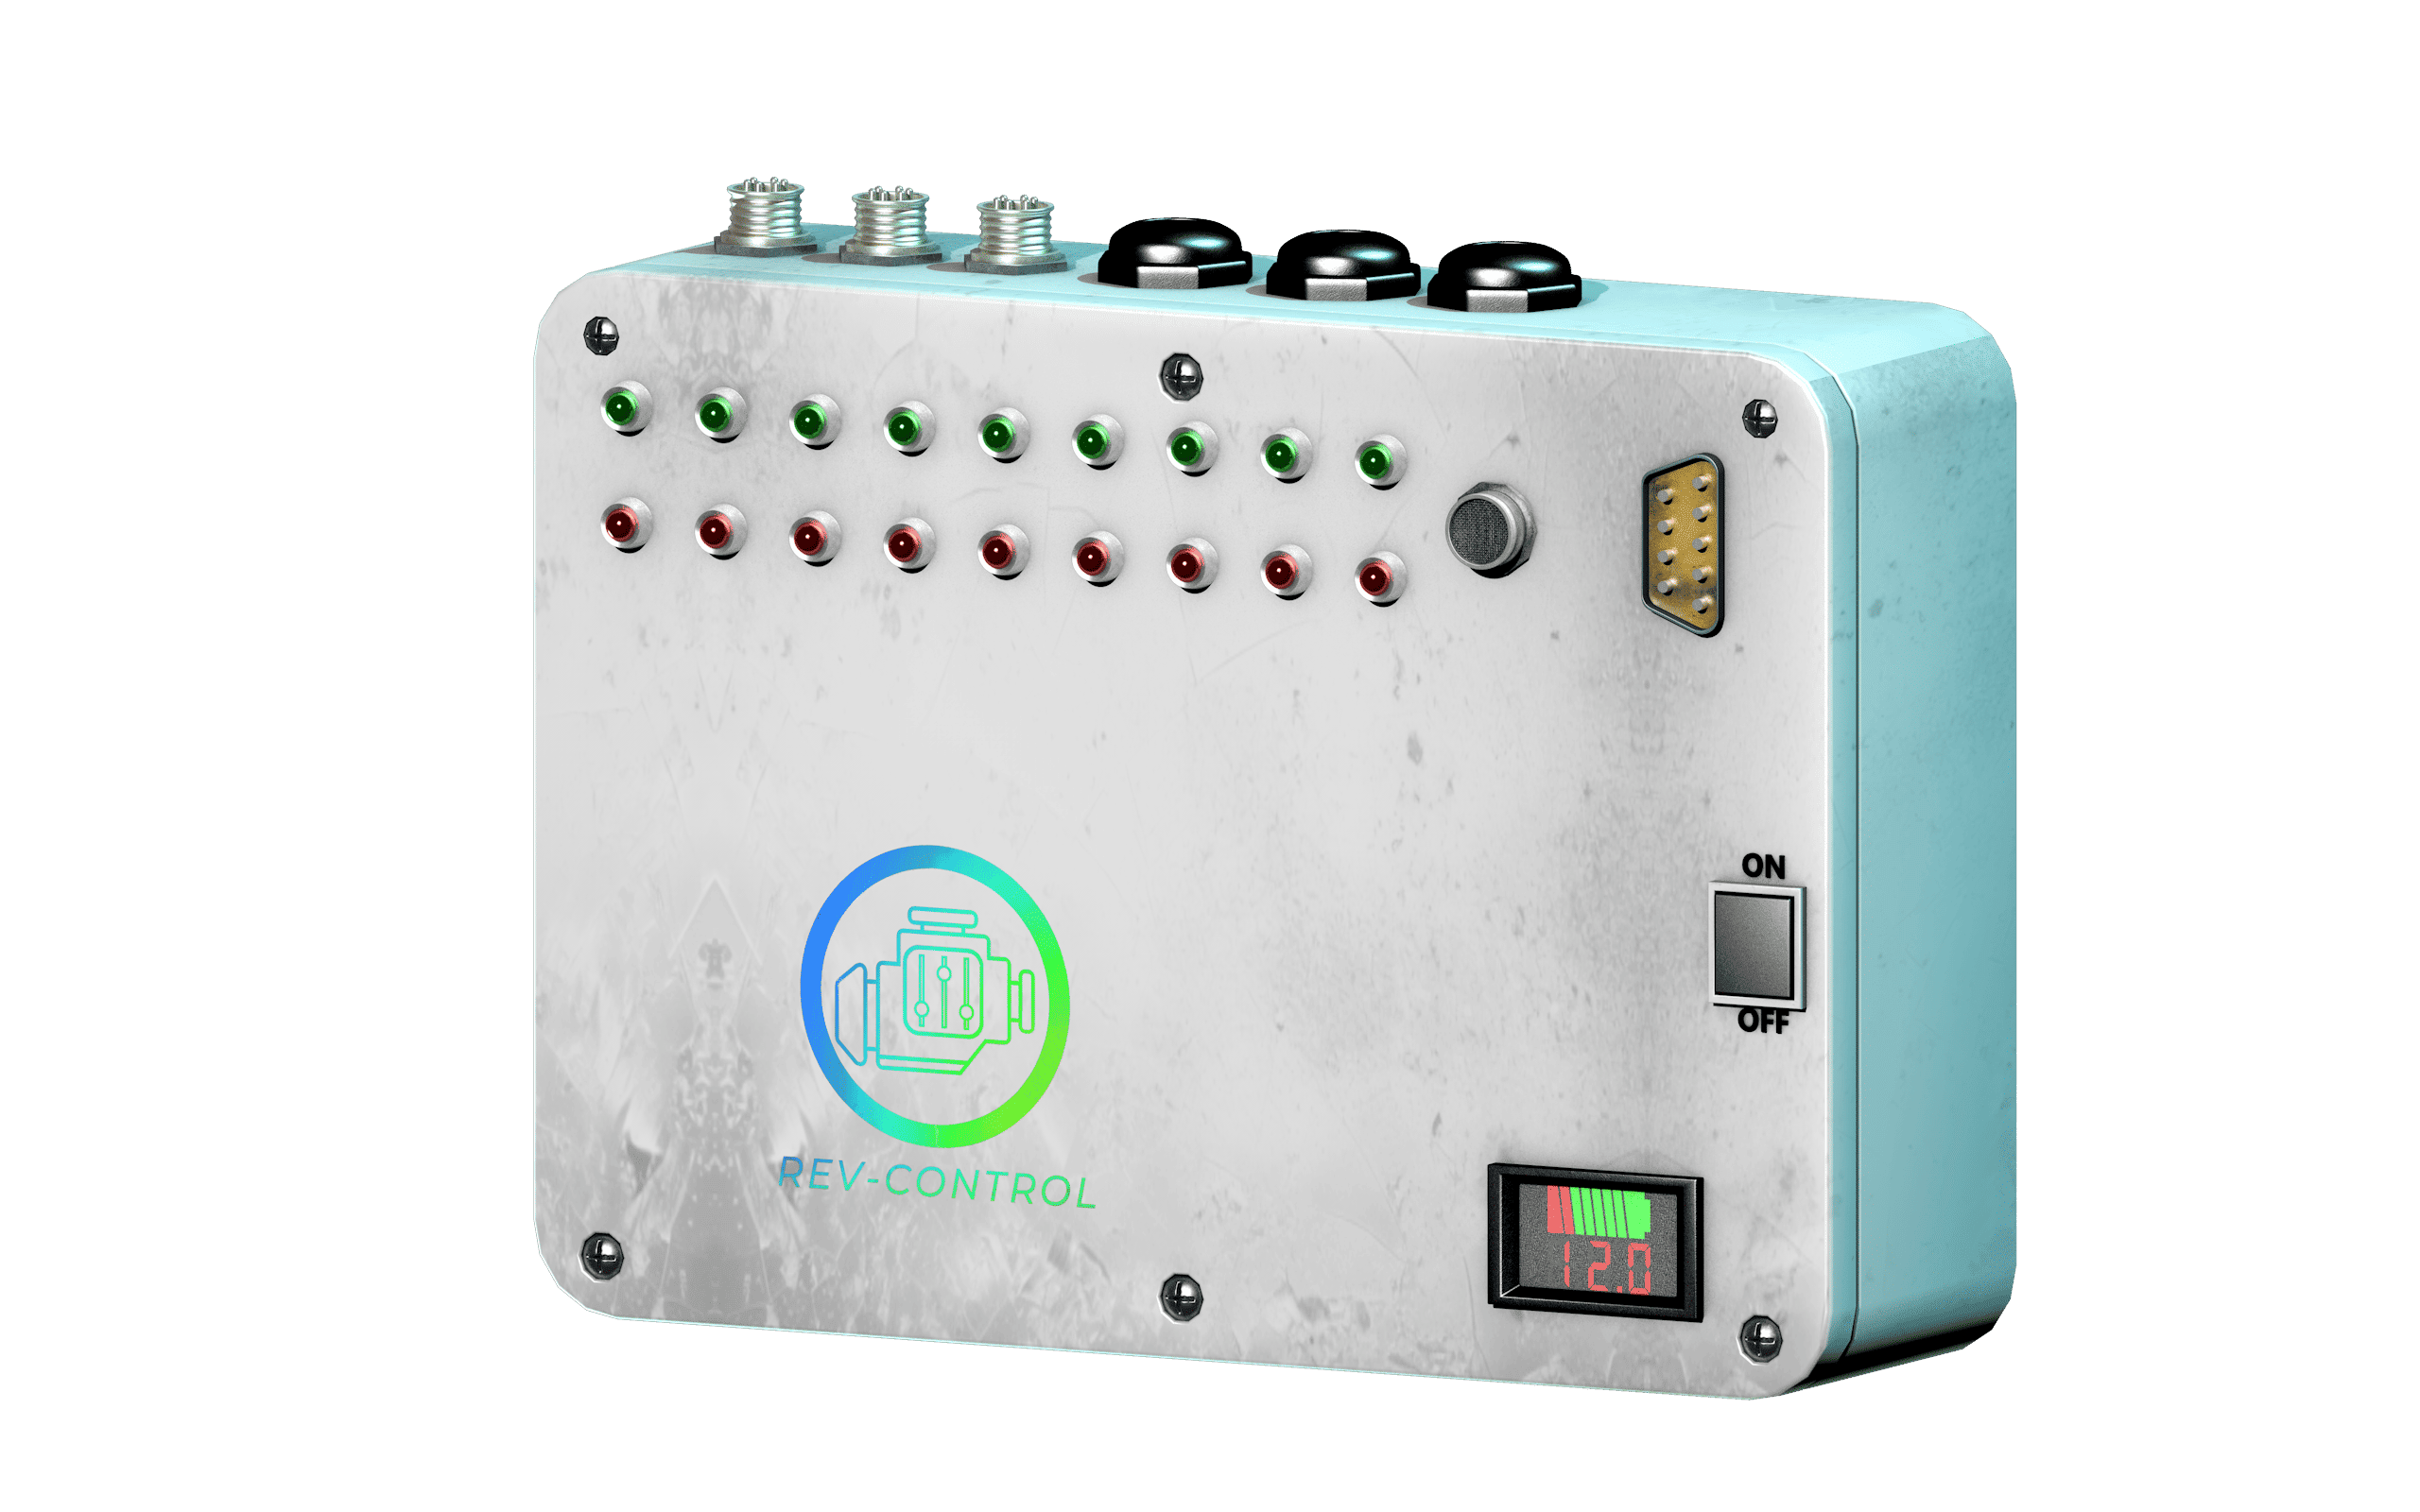
\includegraphics[width=0.8\textwidth]{Imagenes/Tablero rev control.png}
            \captionof{figure}{Módulo de lectura de datos}
            \label{fig:imagen3}
        \end{center}
    \end{itemize}
    
    

% Apéndices
\begin{appendix}
   \chapter{Apéndice A: Esquemáticos}
    El circuito Rev-Control Version 2.6 es un sistema de monitoreo y control de parámetros de un motor, diseñado para la medición y alerta de varias variables como RPM, presión de aceite, temperatura y concentración de oxígeno. Este sistema emplea un microcontrolador LPC845 para gestionar las entradas y salidas de los sensores y se conecta mediante un puerto micro-USB. Utiliza múltiples termocuplas, termistores y sensores específicos conectados a través de amplificadores para cada medición.\\

\begin{enumerate}
    \item \textbf{Microcontrolador LPC845}: Procesa las señales y controla el encendido de alertas. Cuenta con múltiples pines asignados a diferentes sensores y señales de salida.

    \item \textbf{Sensores de Temperatura - Termocuplas (MAX6675)}: Las termocuplas están distribuidas en varias posiciones del sistema para medir temperaturas en puntos específicos, con salidas gestionadas a través de los pines PIO0 del microcontrolador.

    \item \textbf{Sensores de Temperatura - Termistores (MAX31865)}: El MAX31865 convierte las señales de los termistores en datos procesables para el microcontrolador, permitiendo mediciones precisas en otras partes del sistema.

    \item \textbf{Sensor de Presión de Aceite}: Este sensor, conectado a los pines PIO0\_23 y PIO0\_01 del microcontrolador, mide la presión de aceite en el motor, operando en un rango de hasta 7 bar. Permite monitorear la lubricación adecuada del motor, activando alertas en caso de lecturas fuera del rango establecido.

    \item \textbf{Sonda Lambda (\%O2)}: Utiliza el amplificador operacional \textbf{LM358} para ajustar la señal de entrada de la sonda, que mide el nivel de oxígeno en los gases de escape. Indicadores visuales muestran el estado de la medición.

    \item \textbf{Regulador de Voltaje (LD1117D12)}: Proporciona una salida de 3.3V para alimentar componentes de bajo voltaje, asegurando una distribución estable de energía en el sistema.

    \item \textbf{Placa Step Down Regulada a 5V}: Regula la alimentación de 12V a 5V para los componentes que requieren esta tensión, proporcionando una fuente de energía estable y eficiente.

    \item \textbf{Potenciómetro y Resistencias}: Utilizados para calibrar y ajustar las señales de algunos sensores, como la señal de RPM.
\end{enumerate}


    \begin{landscape}
        \begin{sidewaysfigure}
            \centering
            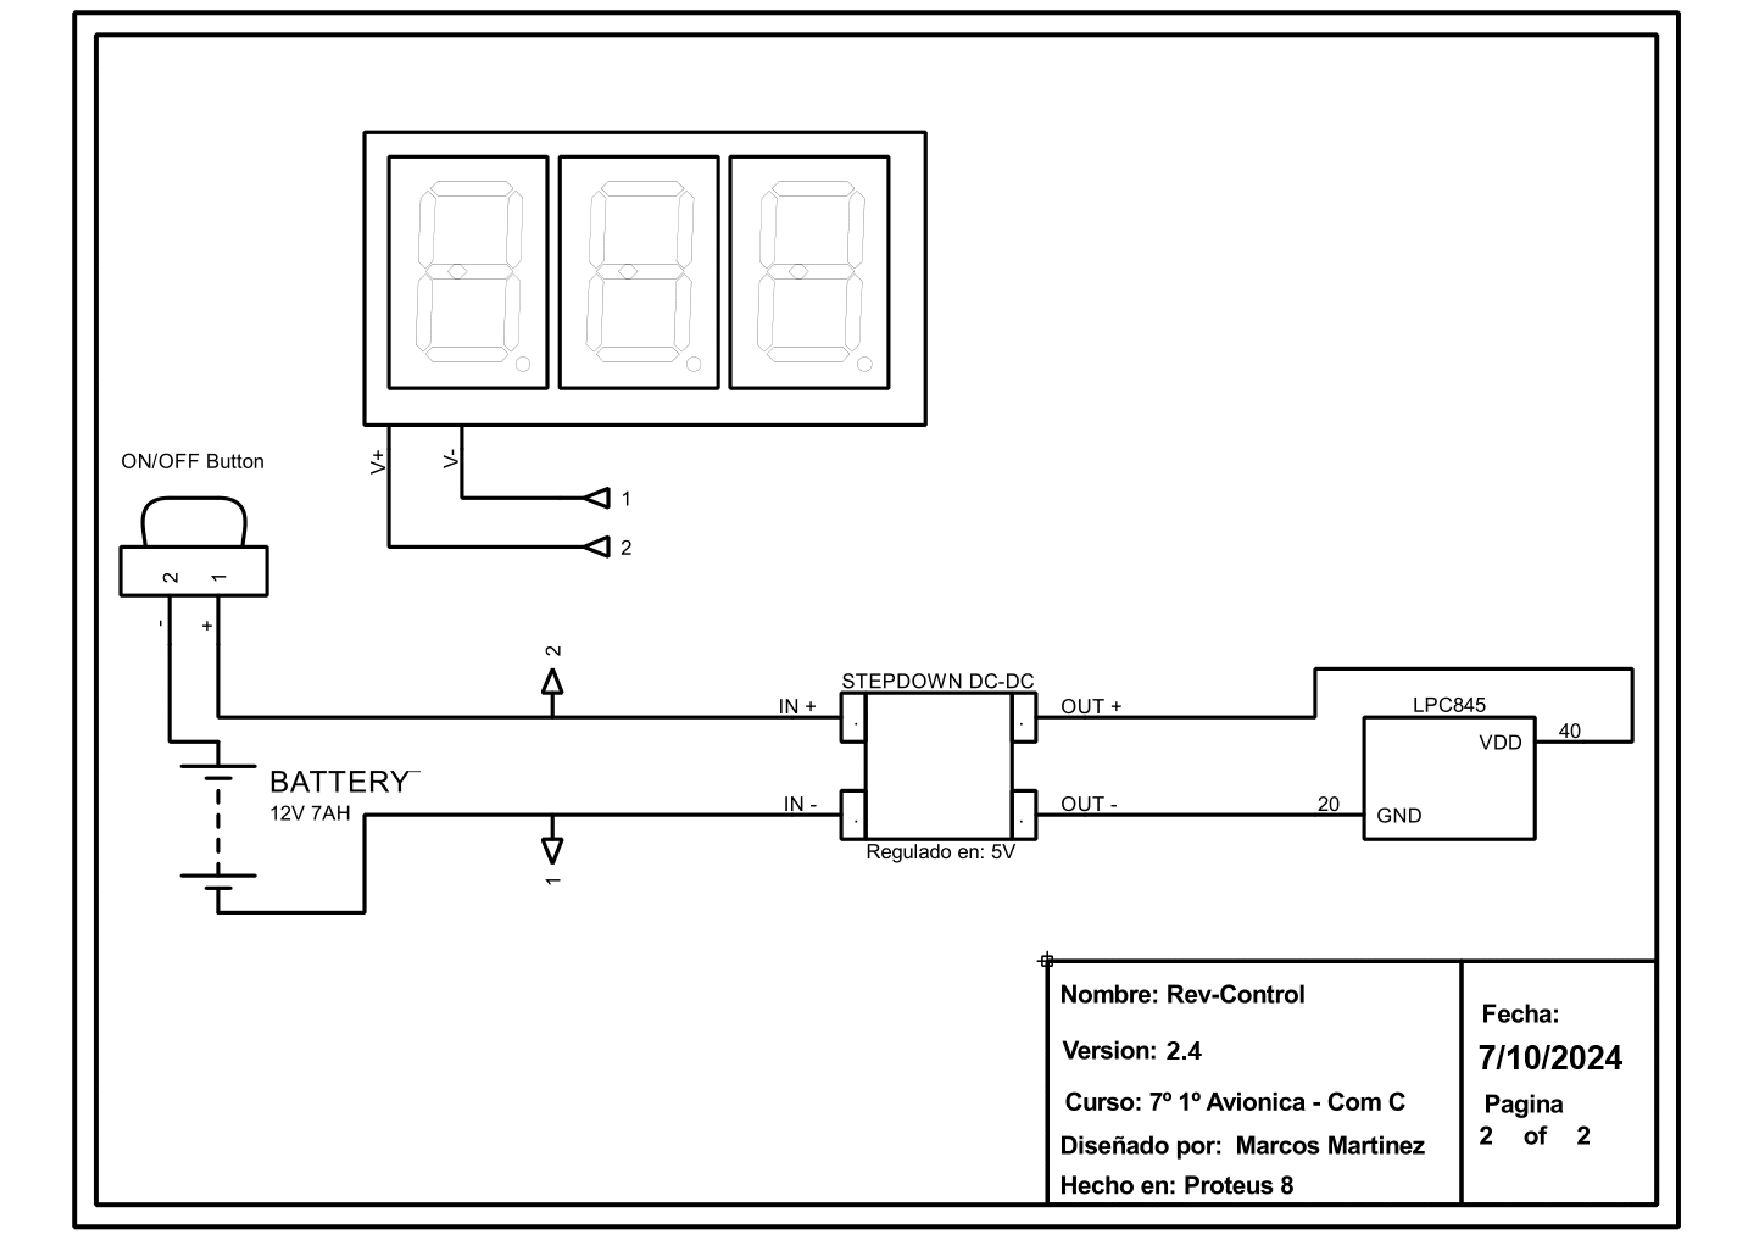
\includegraphics[angle=270, width=\textwidth, keepaspectratio]{Anexo-A Bloque/Rev- Control Version 2.4 Parte 2.pdf}
            \caption{Control Version 2.4 Parte 2}
            \label{fig:A_1}
        \end{sidewaysfigure}
        
        \newpage
        
        \begin{sidewaysfigure}
            \centering
            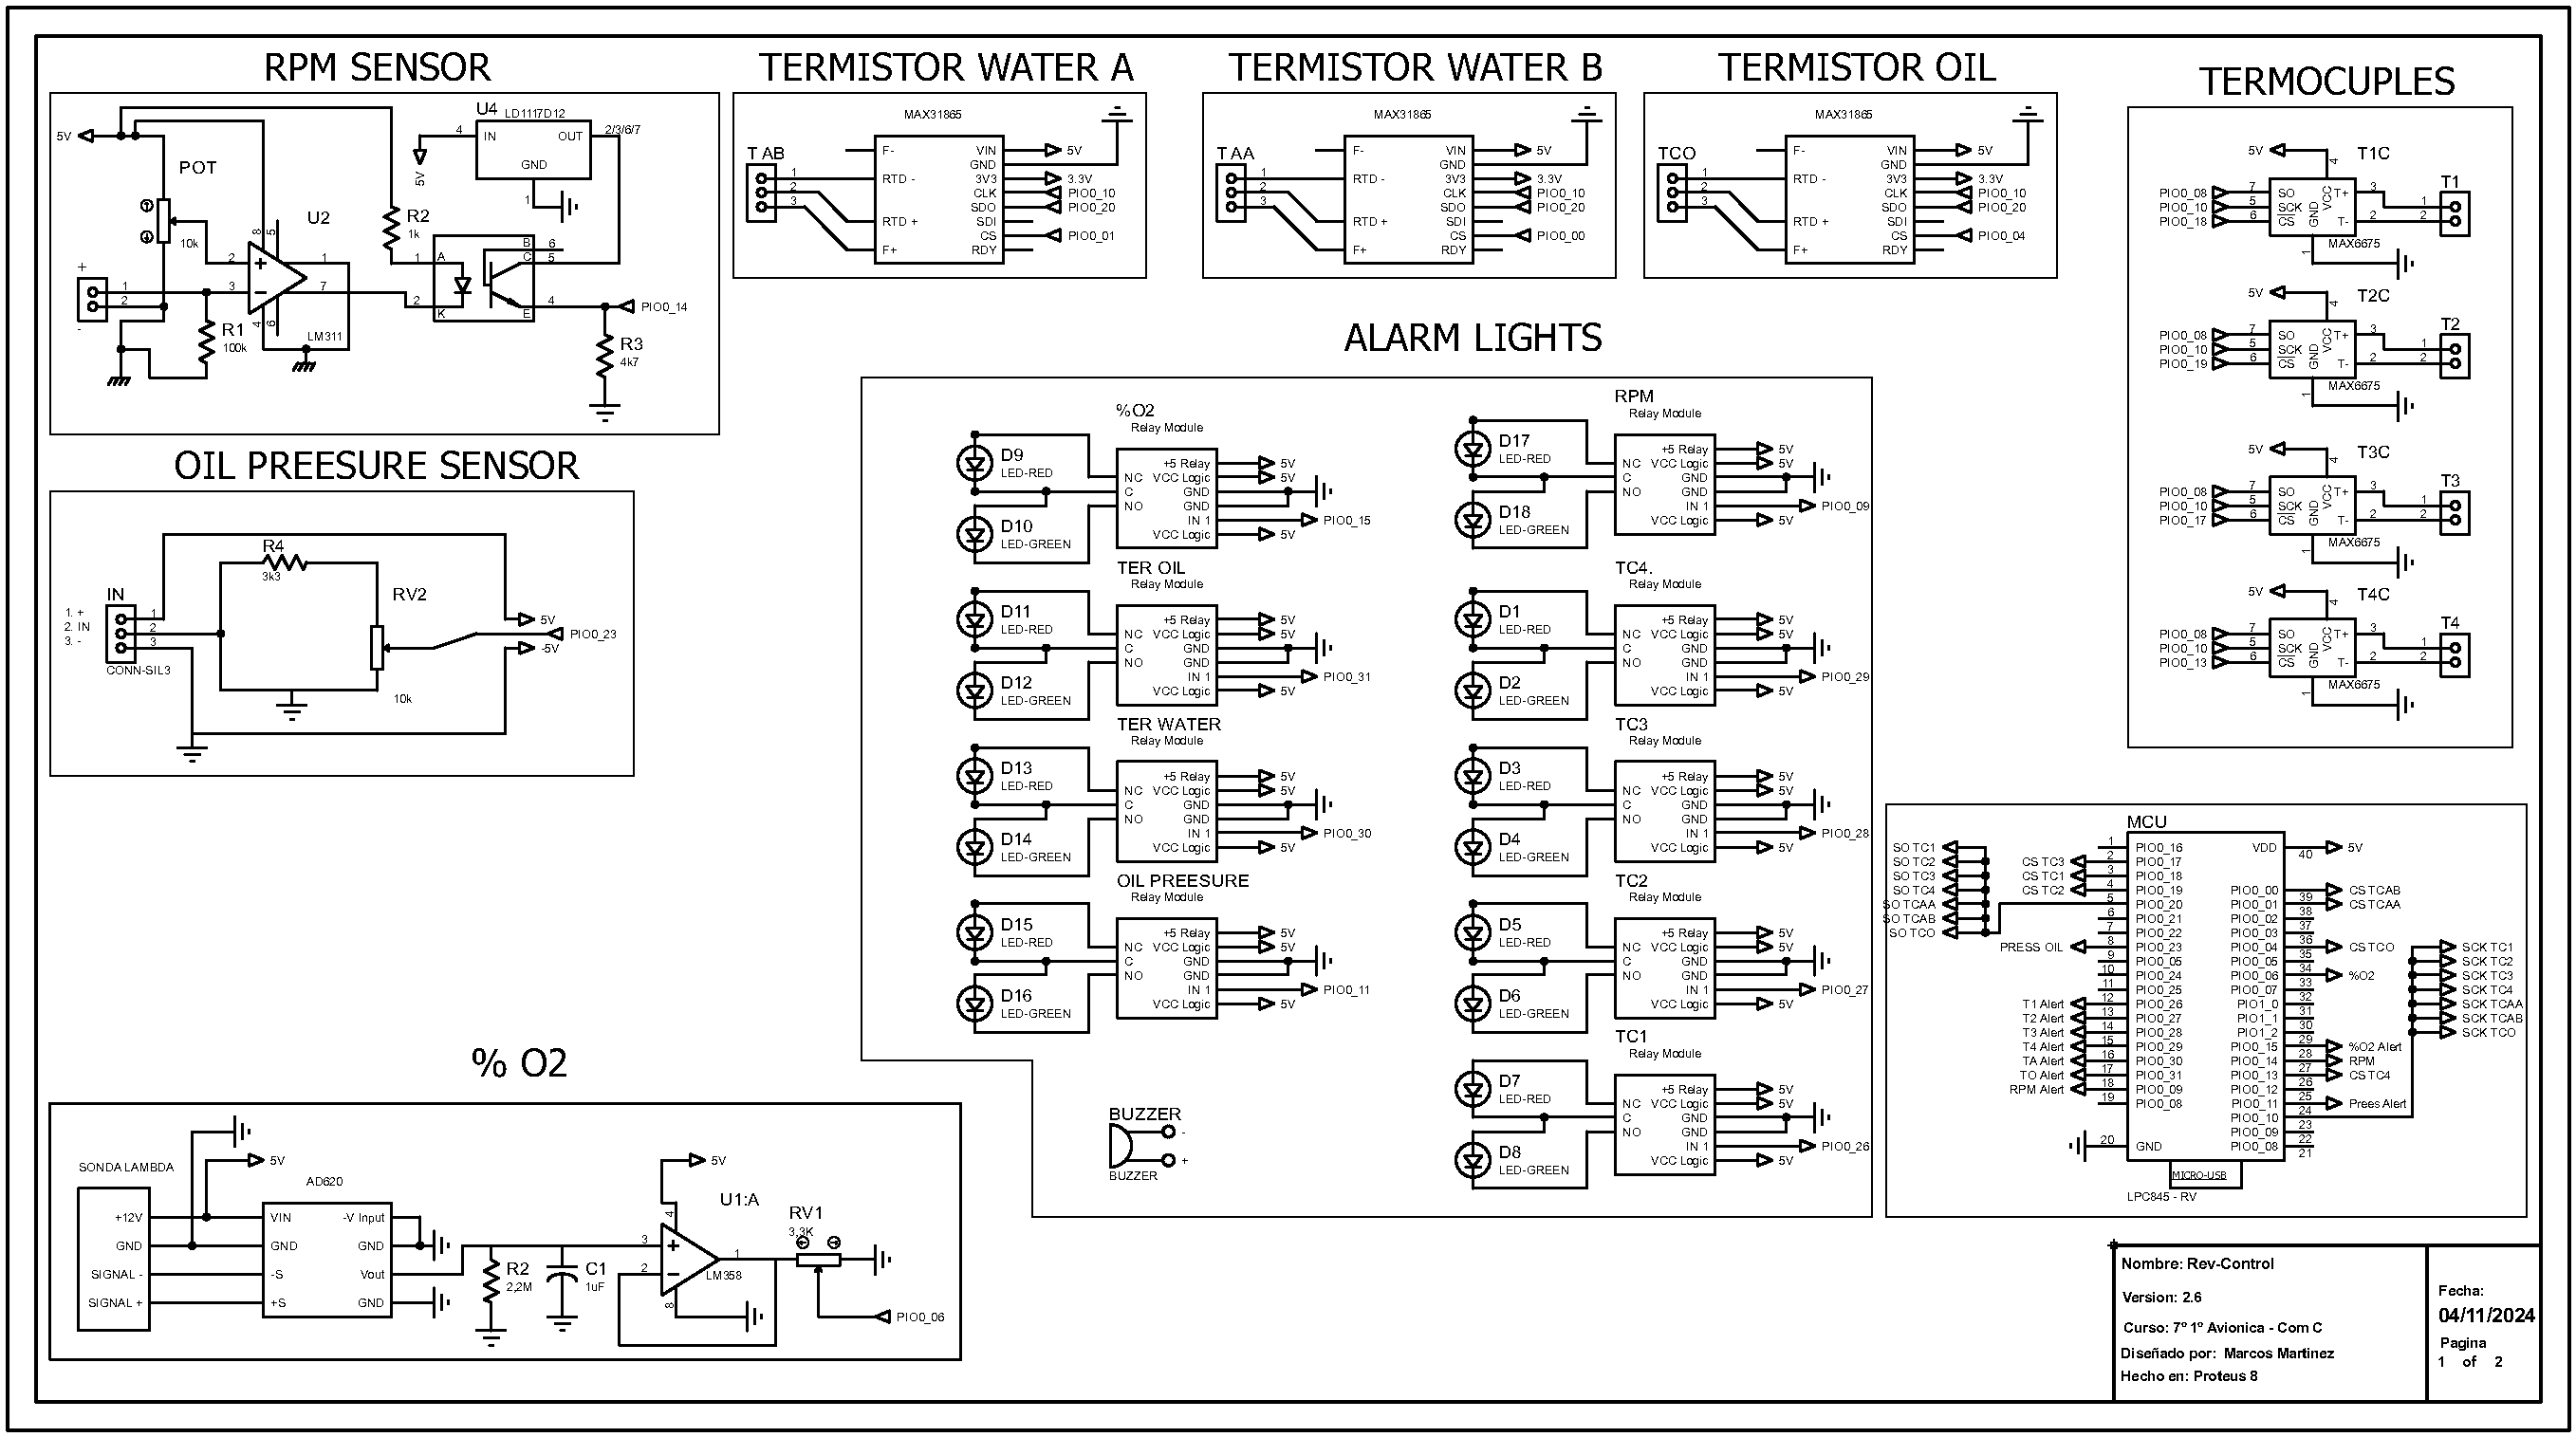
\includegraphics[angle=270, width=\textwidth, keepaspectratio]{Anexo-A Bloque/REV-CONTROL version 2.6.PDF}
            \caption{Control Version 2.6}
            \label{fig:A_2}
        \end{sidewaysfigure}
        
    \end{landscape}
   \chapter{Apéndice B: Documentación-ROTAX}
    La información presentada aquí es el certificado de Aeronavegabilidad y documentación técnica del motor trabajado en este proyecto (Motor ROTAX 912 ULS). Para presentar la bases de información que utilizamos para este proyecto respecto a los parámetros. A continuación se va adjuntar las fuentes de adquisición de dichos documentos y fragmentos de estos mismos:
    
\begin{itemize}
    \item Certificado de Aeronavegabilidad: 
    \hyperlink{certificado-aeronavegabilidad}{-Salto a página-}
    \href{https://www.seguridadaerea.gob.es/sites/default/files/HD%20TC286-I%20r8.pdf}{www.seguridadaerea.gob.es}
    \hfill
     % Enlace directo a la primera página del certificado
    
    \item Documentación Técnica:
    \href{https://www.flyrotax.com/p/service/technical-documentation}{www.flyrotax.com} 

    \begin{itemize}
        \item SERVICE INSTRUCTION - PAC (Pag. 8) 
        \hyperlink{service-instruction-pag8}{-Salto a página-} % Enlace directo a la página 8 en el documento
    \end{itemize}

    \begin{itemize}
        \item MAINTENANCE MANUAL LINE (Pag. 89-90,91-92,88,100,101-103)
        \hyperlink{maintenance-manual-pag91-92}{-Salto a página-} % Enlace directo a la página 91-92 en el documento
    \end{itemize}

    \begin{itemize}
        \item OPERATORS MANUAL LINE (Pag. x)(Pag. 28-29,32)
        \hyperlink{operators-manual1}{-Salto a página-} 
    \end{itemize}

    \begin{itemize}
        \item USER MANUAL (Pag. 35-37) 
        \hyperlink{user-manual}{-Salto a página-} 
    \end{itemize}

    \begin{itemize}
        \item INSTALLATION MANUAL (Pag. 157-158) 
        \hyperlink{manual de instalacion}{-Salto a página-} 
    \end{itemize}
\end{itemize}

% Insertar el PDF completo a continuación de la descripción
\begin{landscape}
    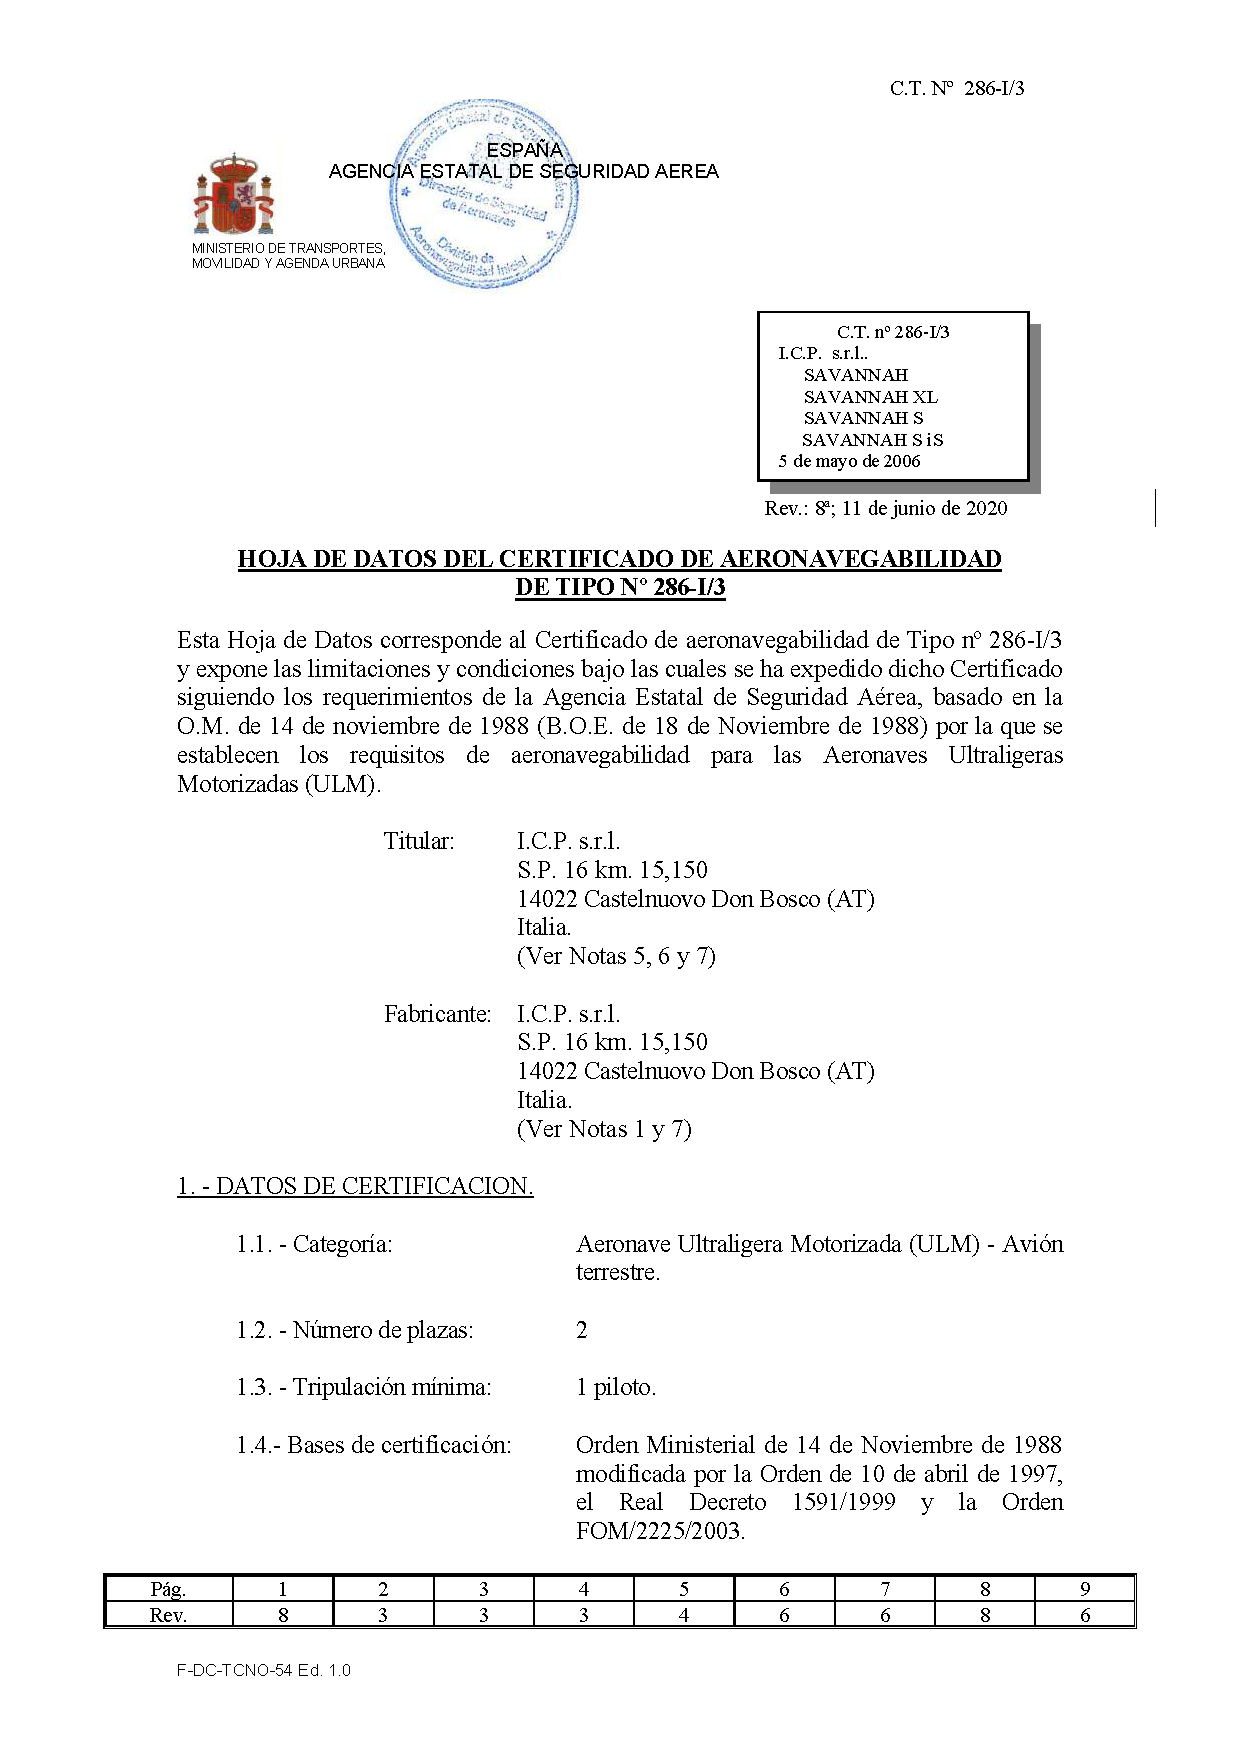
\includepdf[pages=1-2, scale=0.9, pagecommand={\hypertarget{certificado-aeronavegabilidad}{}}]{Anexo-B Bloque/HD TC286-I r8.pdf}
\end{landscape}

\begin{landscape}
    \includepdf[pages=6, scale=0.9, pagecommand={\hypertarget{service-instruction-pag8}{}}]{Anexo-B Bloque/SI-PAC-027.pdf}
\end{landscape}

\begin{landscape}
    
\includepdf[pages={89-90,91-92,88,100,101,102,103}, scale=0.9, pagecommand={\hypertarget{maintenance-manual-pag91-92}{}}]{Anexo-B Bloque/Maintenance Manual Line for Engine Type 912 Series Edition 4 Revision 1.pdf}
\end{landscape}

\begin{landscape}
    
\includepdf[pages={28-29,32}, scale=0.9, pagecommand={\hypertarget{operators-manual1}{}}]{Anexo-B Bloque/OM_912 Series_ED4_R1.pdf}
\end{landscape}

\begin{landscape}
    \includepdf[pages={35-37,28}, scale=0.9, pagecommand={\hypertarget{user-manual}{}}]{Anexo-B Bloque/Manual_Usuario_912.pdf}
\end{landscape}

\begin{landscape}
    \includepdf[pages={157-158}, scale=0.9, pagecommand={\hypertarget{manual de instalacion}{}}]{Anexo-B Bloque/IM_912_Series_Ed3_R0.pdf}
\end{landscape}



\end{appendix}

\end{document}